\chapter{The Four-Rung Ladder}



\ornbreak



\section{The Puzzle of the Vanishing Rules}


I am going to teach you a game. It requires no dice, no board, and no opponents --- only a willingness to watch, with mounting unease, as the rules of arithmetic quietly disintegrate beneath your feet.

Here is how we play. I hand you a number system and a multiplication table. At the first round, the system is small --- just the real numbers you have known since childhood, with their familiar, well-behaved multiplication. At each subsequent round I \textit{double} the size of your number system, constructing a new algebra from the old one by a procedure so mechanical it could be carried out by a clerk in a Victorian counting house. But here is the twist: every time the table doubles, one of the laws of arithmetic --- a law so fundamental you have never questioned it --- silently vanishes. Your job is to spot the missing rule.

Shall we begin?

\textbf{Round 0.} Your system is $\mathbb{R}$, the real numbers. The multiplication table is the one you learned in primary school. Everything works: you can add, subtract, multiply, divide (except by zero), and your numbers line up obediently on a number line from left to right. You can always say which of two numbers is bigger. Life is orderly.

\textbf{Round 1.} I double the reals to obtain $\mathbb{C}$, the complex numbers --- pairs $(a, b)$ of reals, which we write as $a + bi$, where $i^2 = -1$. Your multiplication table has grown from a $1 \times 1$ affair (trivial) to a $2 \times 2$ grid. Everything still \textit{mostly} works. You can add, subtract, multiply, divide. But something is missing. Try to put $3 + 4i$ and $1 - 2i$ in order. Which is "bigger"? The question has no answer. The number line has become a plane, and in a plane there is no natural notion of left and right. \textit{Total ordering has vanished.}

\textbf{Round 2.} I double the complexes to obtain $\mathbb{H}$, the quaternions --- quadruples of reals, which we write as $a + b\mathbf{i} + c\mathbf{j} + d\mathbf{k}$. The multiplication table is now $4 \times 4$. Look carefully at it: is it symmetric about the diagonal? It is not. Compute $\mathbf{i} \cdot \mathbf{j}$ and $\mathbf{j} \cdot \mathbf{i}$ --- they differ by a minus sign. \textit{Commutativity has died.}

\textbf{Round 3.} I double the quaternions to obtain $\mathbb{O}$, the octonions --- eight-tuples of reals, with an $8 \times 8$ multiplication table so intricate it takes a special diagram (the Fano plane) just to remember it. Now try grouping a product of three octonions in different ways: $(x \cdot y) \cdot z$ versus $x \cdot (y \cdot z)$. They are not equal. \textit{Associativity has crumbled.}

\textbf{Round 4.} I double the octonions\index{octonions} to obtain $\mathbb{S}$, the sedenions --- sixteen-tuples. And now something truly catastrophic happens. There exist two \textit{nonzero} sedenions whose product is zero. The division property --- the guarantee that nonzero times nonzero is nonzero --- has collapsed. \textit{The channel breaks.}

\begin{figure}[htbp]
\centering
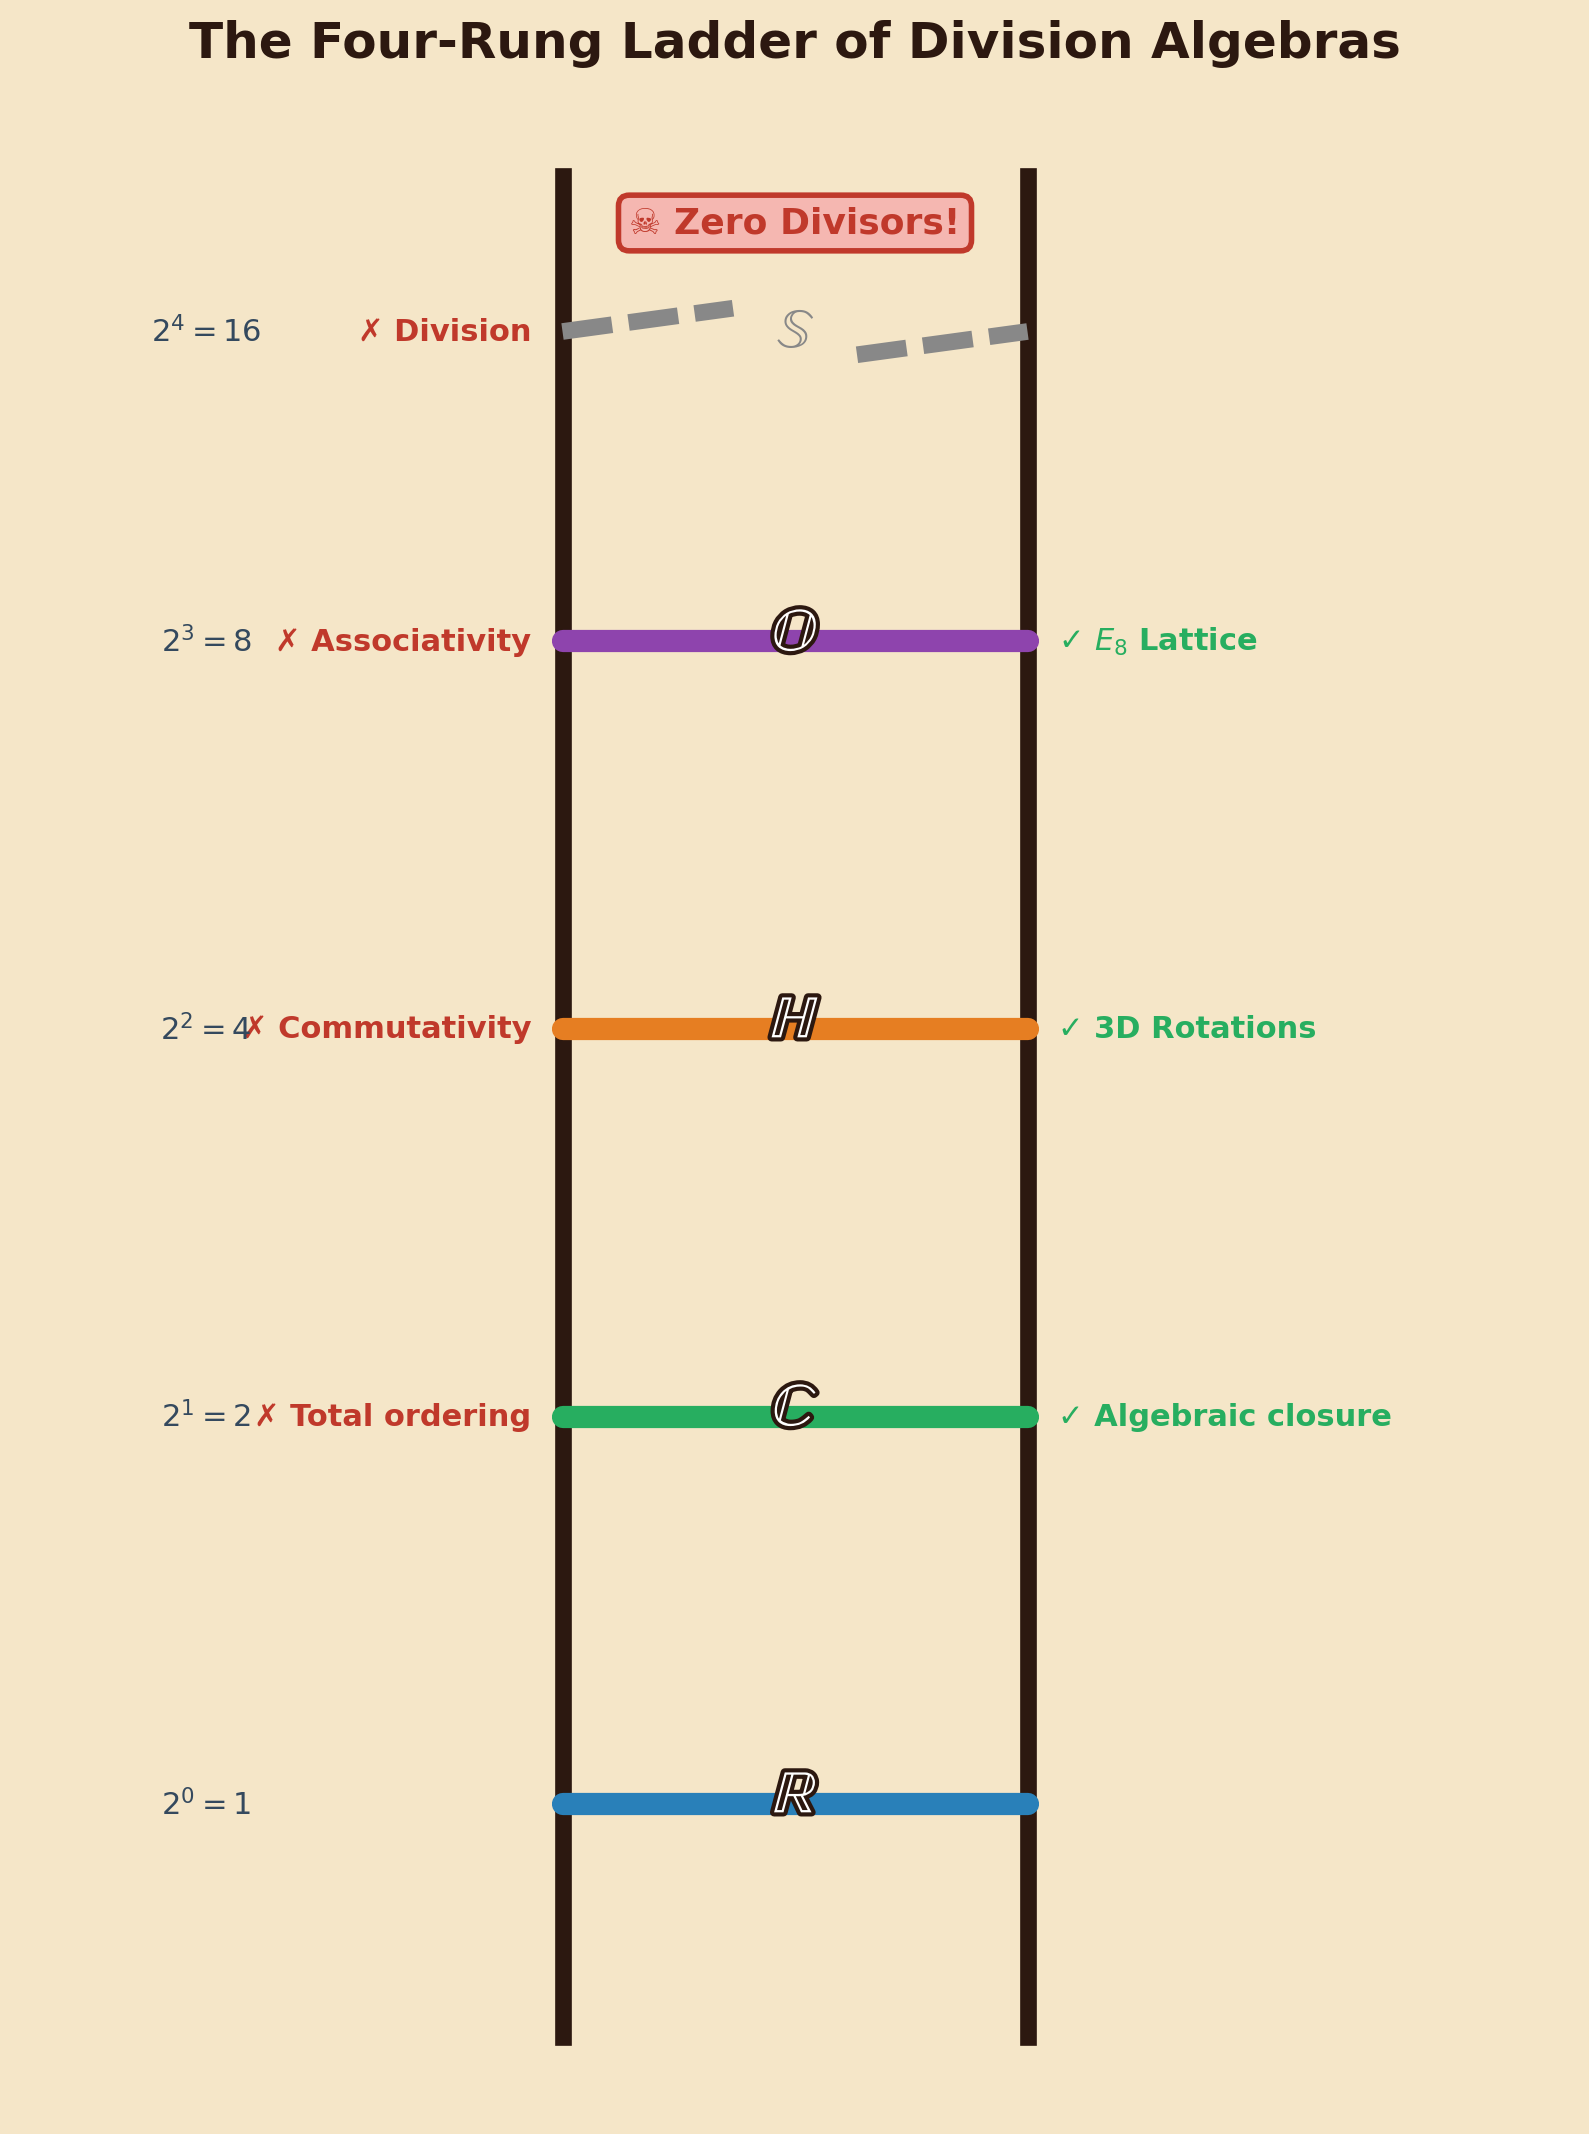
\includegraphics[width=0.82\textwidth,keepaspectratio]{images/chapter9_fig01_four_rung_ladder.png}
\caption{A vertical ladder with exactly four rungs, drawn in a woodcut style.}
\end{figure}


This doubling procedure has a name: it is the \textit{Cayley–Dickson construction}, after Arthur Cayley and Leonard Eugene Dickson, though the idea has roots reaching back to Hamilton himself. The recipe is devastatingly simple. Given any algebra $A$ with a conjugation operation $\bar{a}$, you build a new algebra $A'$ whose elements are pairs $(a, b)$ from $A$, with multiplication defined by:

\[
(a, b) \cdot (c, d) = (ac - \bar{d}b,\; da + b\bar{c}).
\]

Apply this once to $\mathbb{R}$ and you get $\mathbb{C}$. Apply it to $\mathbb{C}$ and you get $\mathbb{H}$. Apply it to $\mathbb{H}$ and you get $\mathbb{O}$. You can keep going forever --- the sedenions, the trigintaduonions, and so on, doubling into the stratosphere --- but each step past the octonions produces an algebra riddled with zero divisors, an arithmetic that has lost the right to call itself a "number system" in any civilized sense.

\begin{figure}[htbp]
\centering
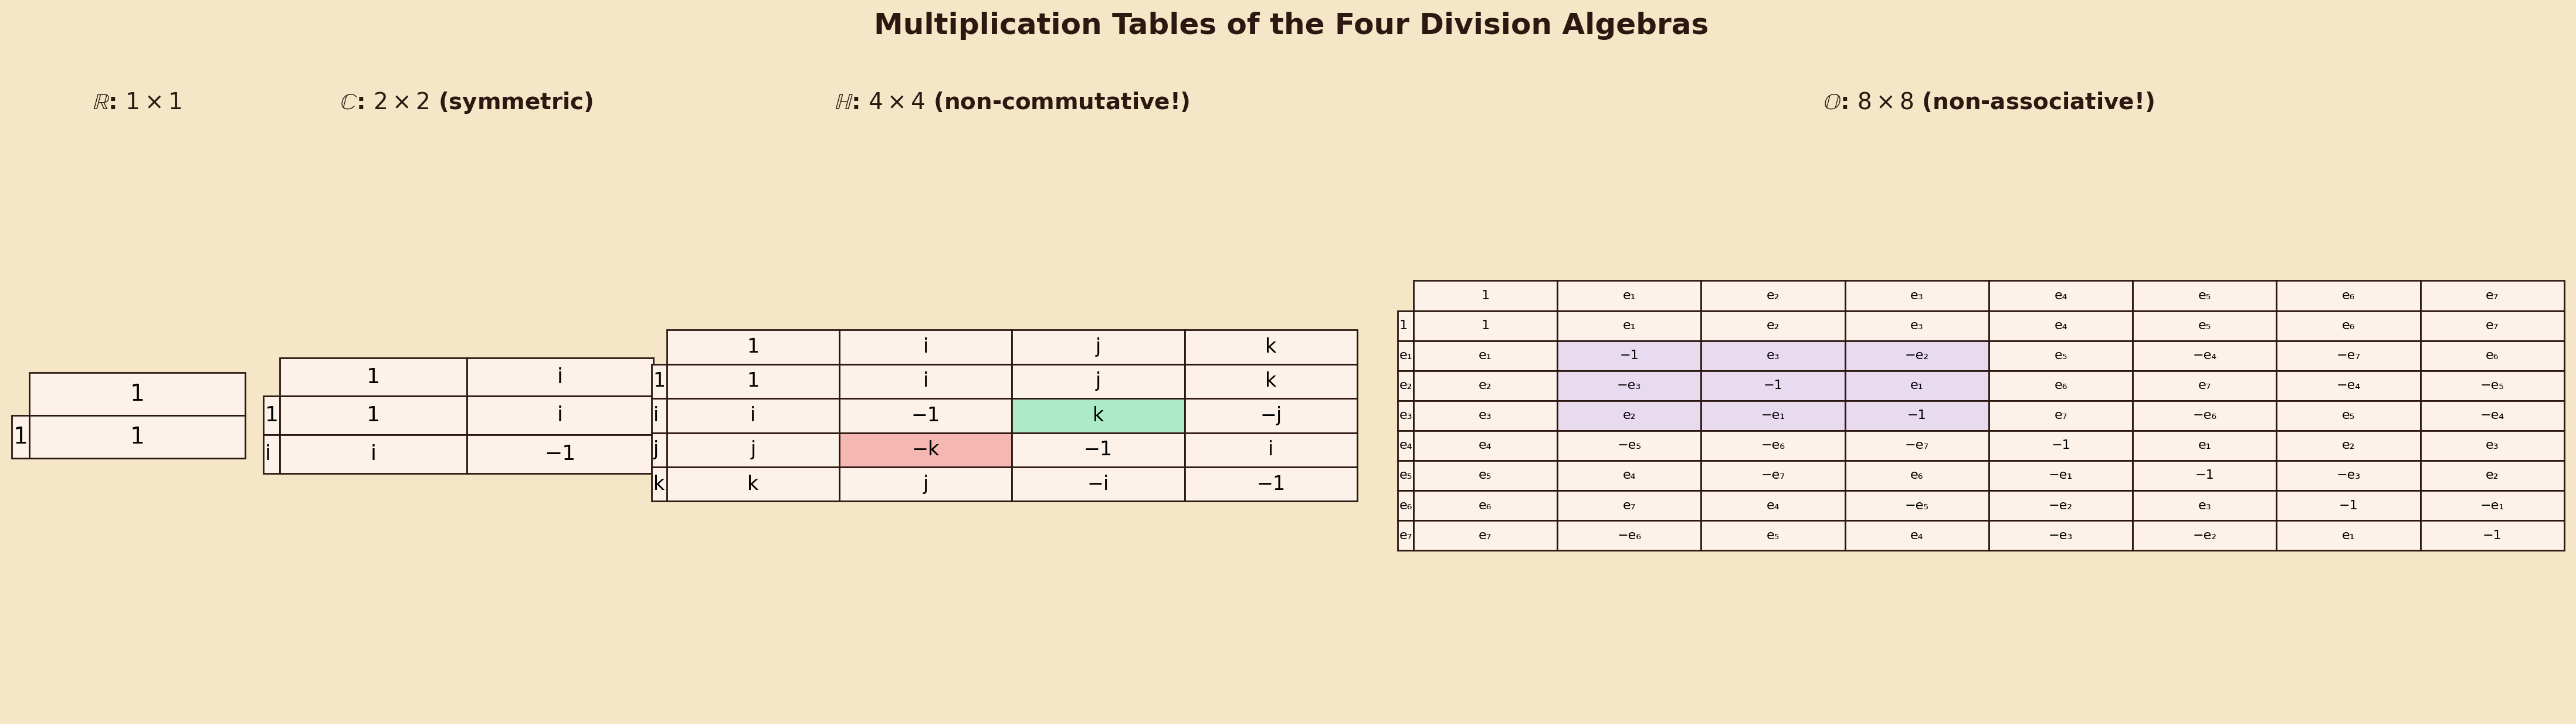
\includegraphics[width=0.82\textwidth,keepaspectratio]{images/chapter9_fig02_multiplication_tables.png}
\caption{Four multiplication tables arranged left-to-right.}
\end{figure}


The story of how these algebras were discovered is one of the great dramas in the history of mathematics. On October 16, 1843, Sir William Rowan Hamilton\index{Hamilton, William Rowan} was walking along the Royal Canal in Dublin when the quaternion multiplication rule burst upon him with such force that he pulled out a knife and carved the equation $i^2 = j^2 = k^2 = ijk = -1$ into the stone of Brougham Bridge. His friend John T. Graves, excited by Hamilton's discovery, promptly invented the octonions --- but Hamilton, distracted by his own creation, sat on Graves's letter for two months, during which Arthur Cayley independently published the same system. Graves spent decades nursing the grievance, and to this day the octonions are sometimes called "Cayley numbers" despite Graves's prior claim. Priority in mathematics, as in love, is a painful business.

But here is the question that will occupy the rest of this chapter: \textit{What do we gain by climbing the ladder? What is the mathematical reward for sacrificing our most cherished algebraic laws?}

The answer, it turns out, lives in the arithmetic of sums of squares --- and it begins with a fact so simple it seems beneath notice.


\ornbreak



\section{The Commutative Paradise --- Why $\mathbb{C}$ Is So Well-Behaved}


Here is a fact so obvious it seems unworthy of mention: $3 \times 5 = 5 \times 3$. Every child knows this. It is the \textit{commutative law} of multiplication, and you have relied on it every time you rearranged factors in an algebraic expression, every time you computed a tip by calculating $0.18 \times 47$ instead of $47 \times 0.18$. The law feels as natural and inevitable as gravity.

But what happens when you graduate from ordinary numbers to the complex plane? Does this kindergarten rule survive the promotion?

Let $z = a + bi$ and $w = c + di$ be two arbitrary complex numbers. Compute:

\[
z \cdot w = (a + bi)(c + di) = ac - bd + (ad + bc)i.
\]

Now swap:

\[
w \cdot z = (c + di)(a + bi) = ca - db + (cb + da)i.
\]

Since real multiplication is commutative --- $ac = ca$, $bd = db$, $ad = da$, $bc = cb$ --- these two expressions are identical. The commutative law survives, perfectly intact, in $\mathbb{C}$.

\textbf{Theorem (Complex Commutativity).} *For all $z, w \in \mathbb{C}$, we have $z \cdot w = w \cdot z$.*

\begin{figure}[htbp]
\centering
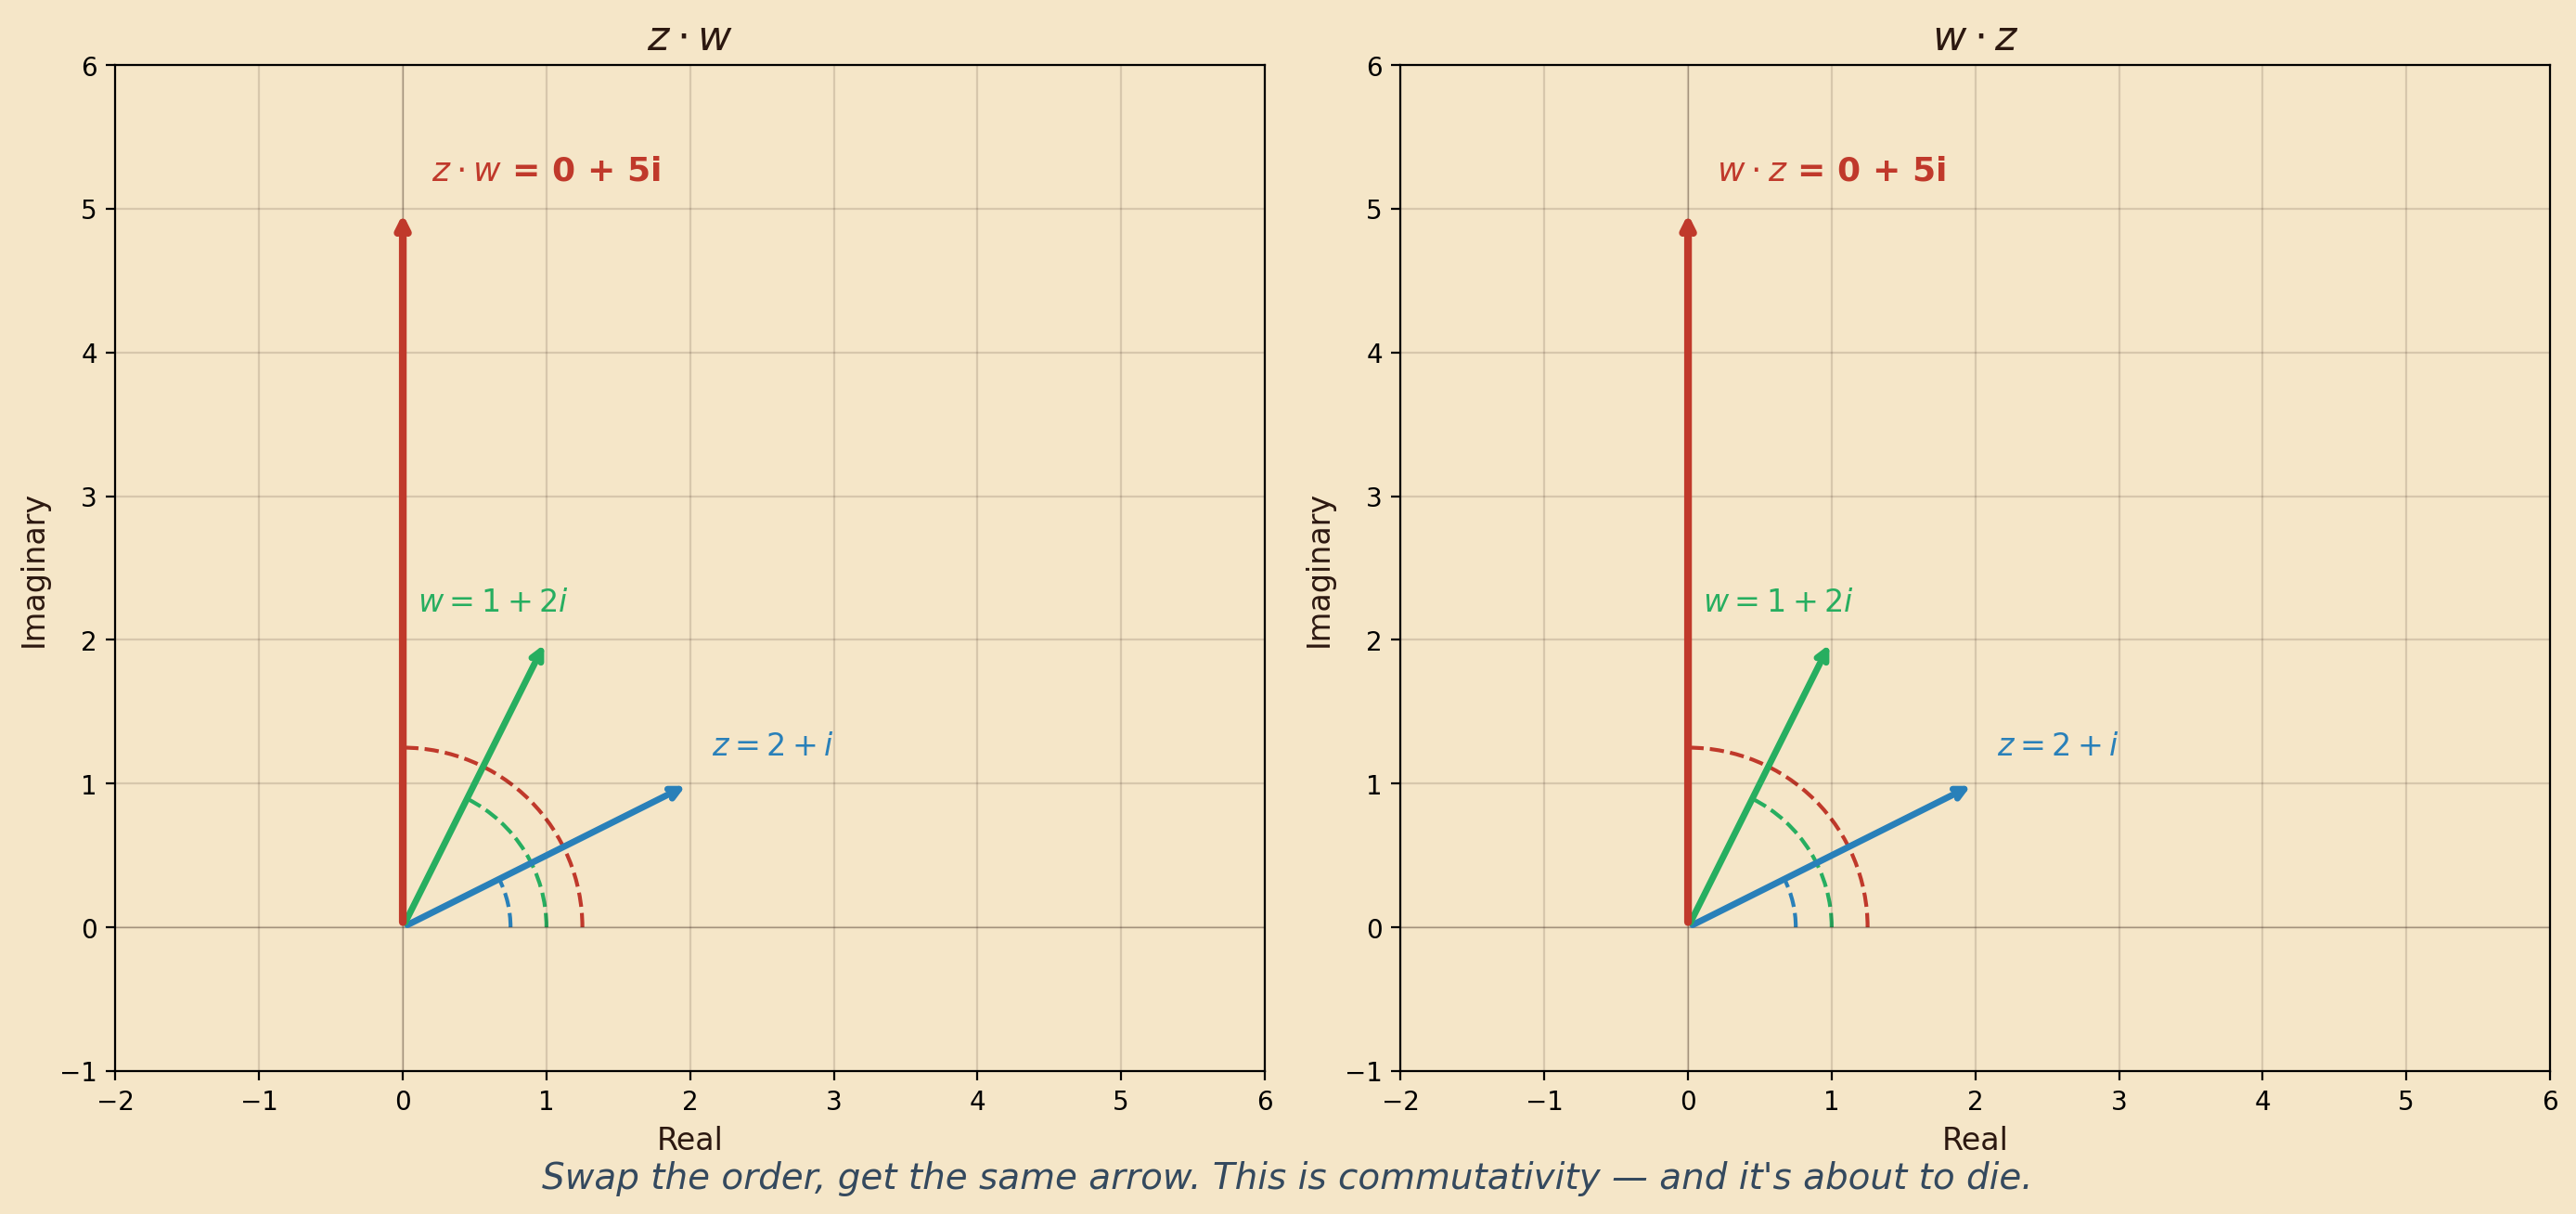
\includegraphics[width=0.82\textwidth,keepaspectratio]{images/chapter9_fig03_argand_commutativity.png}
\caption{Two complex numbers $z$ and $w$ depicted as vectors in the Argand plane.}
\end{figure}


The proof has a lovely geometric interpretation. Multiplying by a complex number $z$ does two things to the plane: it \textit{scales} by $|z|$ and \textit{rotates} by $\arg(z)$. Since scaling factors multiply (no matter the order) and rotation angles add (and addition of real numbers is commutative), the composite operation doesn't care which factor comes first. The complex numbers are, in a precise sense, the \textit{last safe harbor} --- the largest Cayley–Dickson algebra where you can freely rearrange the factors in a product. Beyond $\mathbb{C}$, the commutative paradise is lost, and you must watch your step.

This seemingly obvious result is the foundation for everything that follows. The fact that $z \cdot w = w \cdot z$ is what makes the Brahmagupta\index{Brahmagupta}–Fibonacci identity work so smoothly, as we are about to see.


\ornbreak



\section{The Norm That Multiplies --- Brahmagupta's Ancient Gift}


Here is a party trick worthy of a seventh-century Indian mathematician. Pick any two numbers, each of which is a sum of two perfect squares. Multiply them together. I claim the result is \textit{also} a sum of two squares --- and I can tell you \textit{which} ones.

Let us try it. Take $5 = 1^2 + 2^2$ and $13 = 2^2 + 3^2$. Their product is $5 \times 13 = 65$. Now, is $65$ a sum of two squares? A moment's rummaging turns up two representations: $65 = 4^2 + 7^2 = 1^2 + 8^2$. Splendid. But was this a lucky accident, or is there a general rule?

There is a general rule, and it was known to Brahmagupta of Ujjain, who recorded it in his \textit{Brāhmasphuṭasiddhānta} in the year 628 CE --- more than five centuries before Fibonacci rediscovered it in Europe:

\textbf{Theorem (Brahmagupta–Fibonacci Identity).}

\[
(a^2 + b^2)(c^2 + d^2) = (ac - bd)^2 + (ad + bc)^2.
\]

The proof is pure algebra. Expand the right side:

\[
(ac - bd)^2 + (ad + bc)^2 = a^2c^2 - 2abcd + b^2d^2 + a^2d^2 + 2abcd + b^2c^2
\]
\[
= a^2c^2 + a^2d^2 + b^2c^2 + b^2d^2 = (a^2 + b^2)(c^2 + d^2).
\]

The $-2abcd$ and $+2abcd$ terms cancel --- a small miracle of sign management --- and everything collapses to the product on the left. $\blacksquare$

\begin{figure}[htbp]
\centering
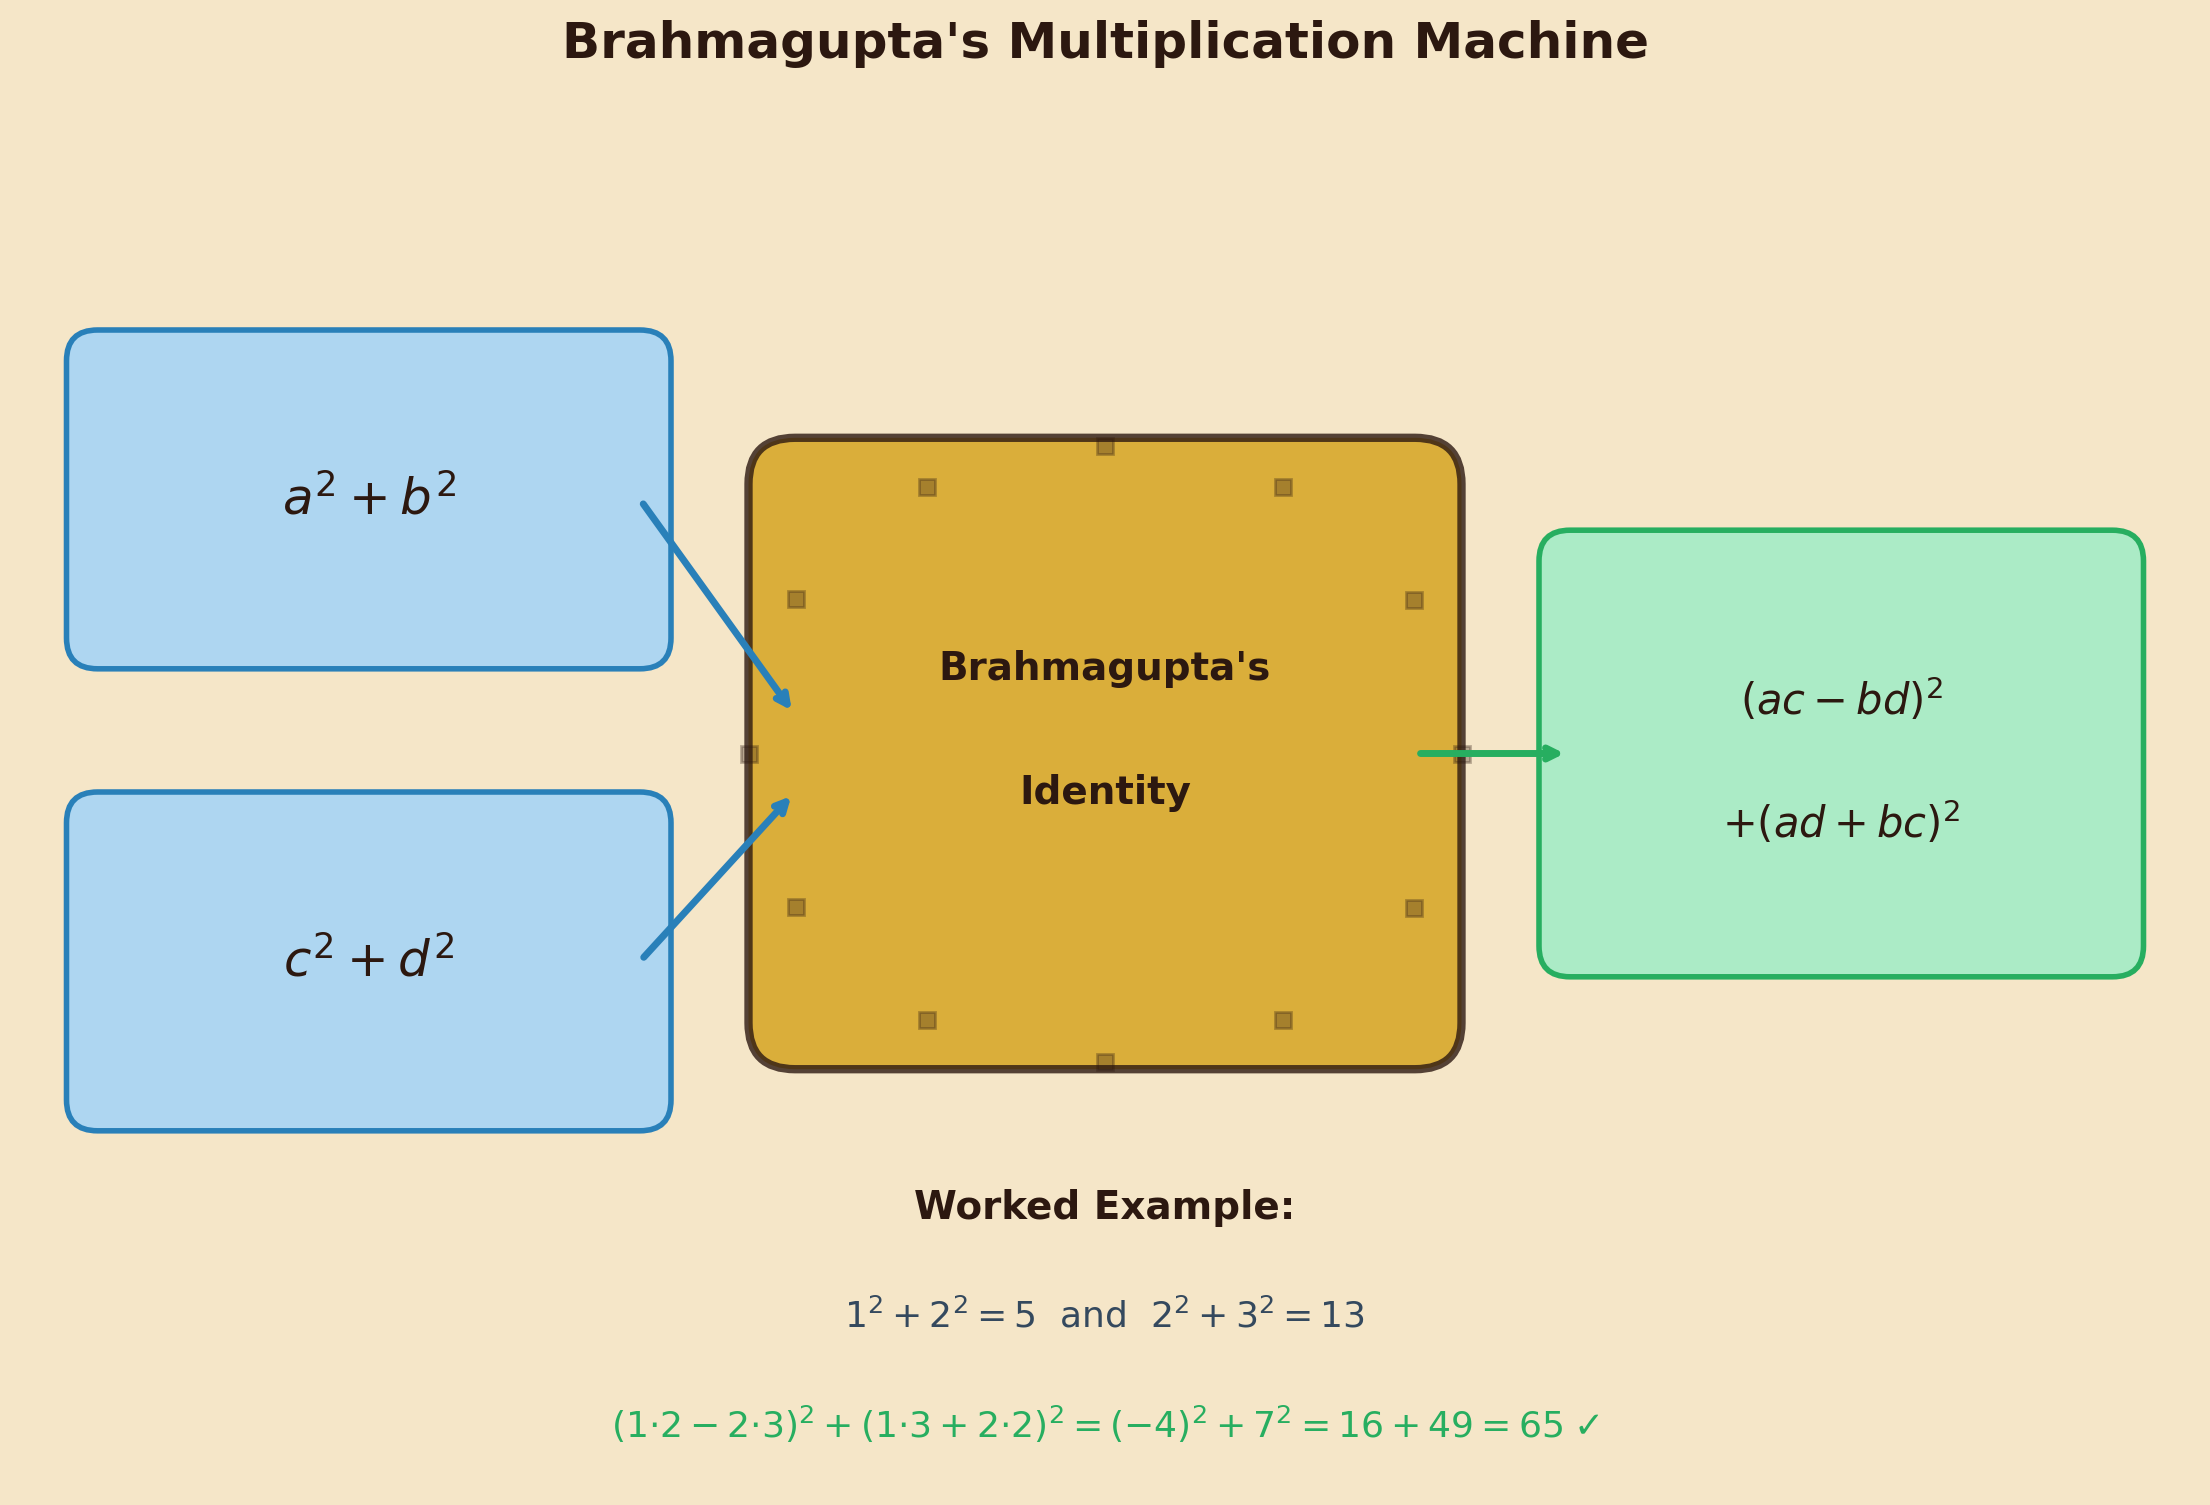
\includegraphics[width=0.82\textwidth,keepaspectratio]{images/chapter9_fig04_brahmagupta_machine.png}
\caption{A visual "multiplication machine." Two input boxes on the left are labeled "$a^2 + b^2$" and "$c^2 + d^2$." An arrow feeds them into a gearbox labeled "Brahmagupta's Identity." Out the right side emerges a single box labeled "$(ac - bd)^2 + (ad + bc)^2$." Below, a worked numerical example: inputs $1^2 + 2^2 = 5$ and $2^2 + 3^2 = 13$, output $(1\cdot 2 - 2\cdot 3)^2 + (1\cdot 3 + 2\cdot 2)^2 = (-4)^2 + 7^2 = 16 + 49 = 65$.}
\end{figure}


Now here is the punchline that connects this ancient identity to our ladder of algebras. If we set $z = a + bi$ and $w = c + di$, then the \textit{norm-squared} of a complex number is $|z|^2 = a^2 + b^2$. The Brahmagupta–Fibonacci identity is simply the statement:

\[
|z \cdot w|^2 = |z|^2 \cdot |w|^2.
\]

In other words, the norm on $\mathbb{C}$ is \textit{multiplicative}. The norm of a product equals the product of the norms. This is the "composition algebra property" --- the defining feature that makes $\mathbb{C}$ a \textit{composition algebra} over $\mathbb{R}$.

The historical journey of this identity is a saga in miniature. From Brahmagupta's Sanskrit treatise, it traveled westward through Arabic translations, reached Leonardo of Pisa (Fibonacci) around 1225, and became a workhorse in Euler\index{Euler, Leonhard}'s number theory in the eighteenth century. Euler used it relentlessly in his investigations of which primes can be written as sums of two squares --- and it was Euler who first wondered whether the trick could be extended to sums of \textit{four} squares. That question would take another century to answer, and the answer would arrive from the most unexpected direction: a knife, a canal, and an act of algebraic vandalism on an Irish bridge.


\ornbreak



\section{The Day Commutativity Died --- Hamilton and the Quaternions}


On October 16, 1843, Sir William Rowan Hamilton was walking along the towpath of the Royal Canal in Dublin, accompanying his wife to a meeting of the Royal Irish Academy. He had been obsessed, for more than a decade, with a single question: \textit{Can you build a number system that does for three-dimensional space what the complex numbers do for the plane?}

The complex numbers let you encode two-dimensional rotations as multiplications: multiplying by $e^{i\theta}$ rotates a vector by angle $\theta$. Hamilton wanted a system of "triplets" --- three-component numbers --- that would encode three-dimensional rotations the same way. He tried every algebraic structure he could imagine. He tried for \textit{thirteen years}. His wife, Lady Hamilton, took to asking him at breakfast every morning: "Well, dear, can you multiply triplets yet?" Every morning, the answer was the same: "No, I can only add and subtract them."

The revelation that struck him on Brougham Bridge was that triplets were a dead end. To capture three-dimensional rotations, you need not \textit{three} but \textit{four} components. Hamilton scrawled the defining equations on the bridge with his penknife:

\[
\mathbf{i}^2 = \mathbf{j}^2 = \mathbf{k}^2 = \mathbf{i}\mathbf{j}\mathbf{k} = -1.
\]

From these three relations, the entire multiplication table follows --- and it contains a shock. Let us compute $\mathbf{i} \cdot \mathbf{j}$. From $\mathbf{i}\mathbf{j}\mathbf{k} = -1$, multiply both sides on the right by $\mathbf{k}$:

\[
\mathbf{i}\mathbf{j}\mathbf{k}^2 = -\mathbf{k}, \quad \text{so} \quad \mathbf{i}\mathbf{j}(-1) = -\mathbf{k}, \quad \text{so} \quad \mathbf{i}\mathbf{j} = \mathbf{k}.
\]

Now compute $\mathbf{j} \cdot \mathbf{i}$. Multiply $\mathbf{i}\mathbf{j}\mathbf{k} = -1$ on the left by $\mathbf{i}$ and use $\mathbf{i}^2 = -1$:

\[
-\mathbf{j}\mathbf{k} = -\mathbf{i}, \quad \text{so} \quad \mathbf{j}\mathbf{k} = \mathbf{i}.
\]

Then multiply $\mathbf{i}\mathbf{j}\mathbf{k} = -1$ on the left by $\mathbf{j}$:

\[
\mathbf{j}\mathbf{i}\mathbf{j}\mathbf{k} = -\mathbf{j}, \quad \text{and using } \mathbf{j}^2 = -1: \quad -\mathbf{i}\mathbf{j}\mathbf{k} = -\mathbf{j}.
\]

More directly, since $\mathbf{i}\mathbf{j} = \mathbf{k}$, we can test: if commutativity held, we would have $\mathbf{j}\mathbf{i} = \mathbf{k}$ as well. But then $\mathbf{j}\mathbf{i}\mathbf{j}\mathbf{i} = \mathbf{k}^2 = -1$. Yet also $\mathbf{j}\mathbf{i}\mathbf{j}\mathbf{i} = \mathbf{j}(\mathbf{i}\mathbf{j})\mathbf{i} = \mathbf{j}\mathbf{k}\mathbf{i} = \mathbf{i} \cdot \mathbf{i} = -1$... the contradiction is hiding, so let us simply \textit{compute directly}. Using the full multiplication table derived from Hamilton's axioms:

\[
\mathbf{j} \cdot \mathbf{i} = -\mathbf{k}.
\]

\textbf{Theorem (Quaternion Non-Commutativity).} *There exist $a, b \in \mathbb{H}$ such that $a \cdot b \neq b \cdot a$.*

\textit{Proof.} Take $a = \mathbf{i} = (0, 1, 0, 0)$ and $b = \mathbf{j} = (0, 0, 1, 0)$. Then $\mathbf{i}\mathbf{j} = \mathbf{k} = (0, 0, 0, 1)$, while $\mathbf{j}\mathbf{i} = -\mathbf{k} = (0, 0, 0, -1)$. In the fourth component, $1 \neq -1$, so the products are distinct. $\blacksquare$

\begin{figure}[htbp]
\centering
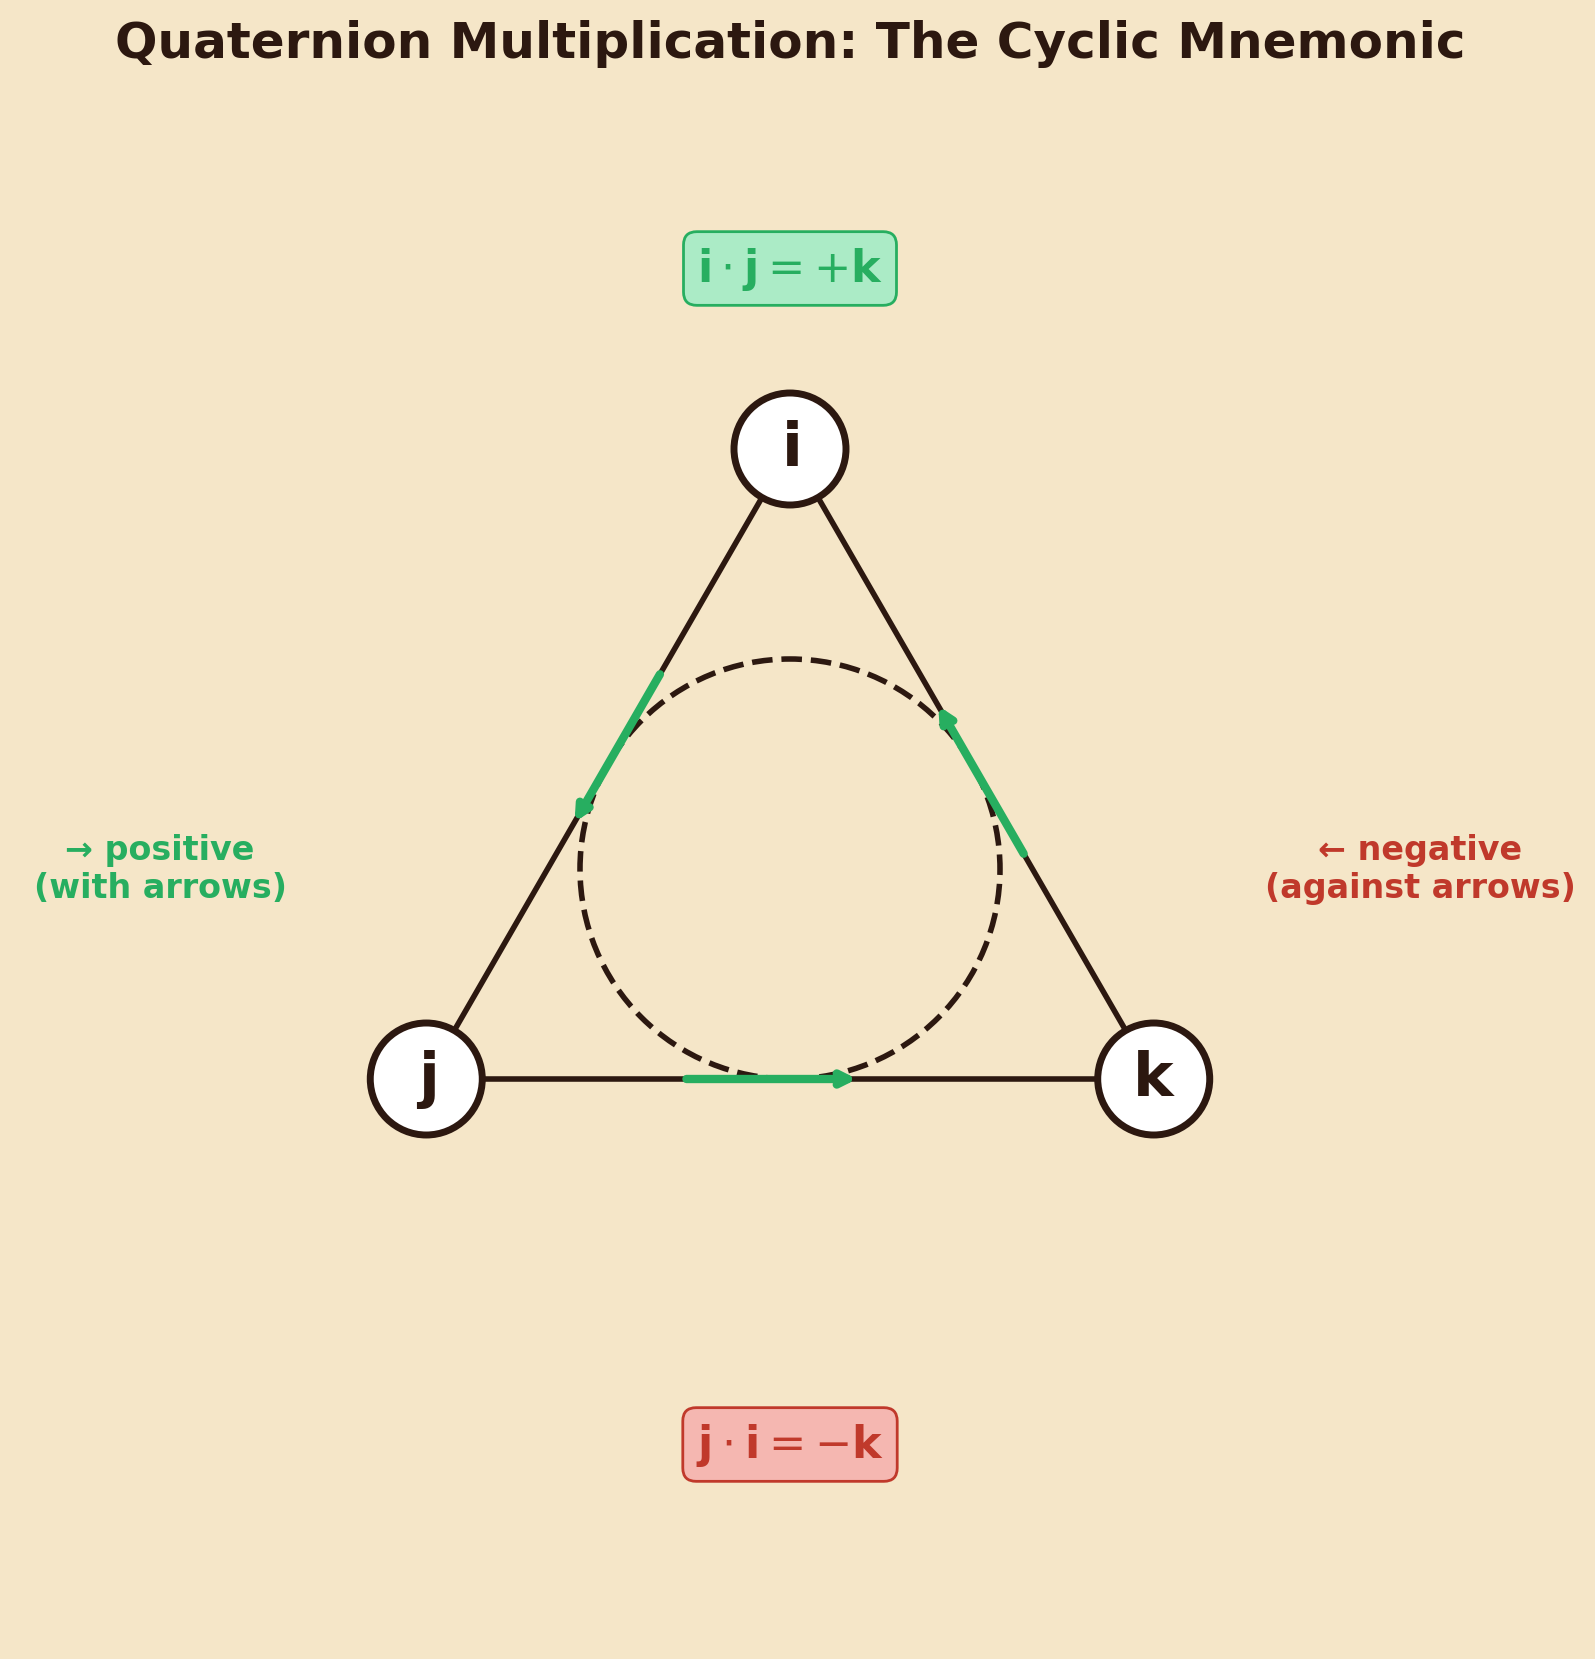
\includegraphics[width=0.82\textwidth,keepaspectratio]{images/chapter9_fig05_quaternion_fano.png}
\caption{The famous Fano-plane mnemonic for quaternion multiplication.}
\end{figure}


What does commutativity's death \textit{buy} us? Try this experiment at home. Take a book and hold it flat, cover facing you. First rotate it $90°$ about the horizontal axis (the book now faces the ceiling), then $90°$ about the vertical axis (the book now faces to your left). Return to the starting position and reverse the order: first the vertical rotation, then the horizontal. The book now faces in a completely different direction.

\begin{figure}[htbp]
\centering
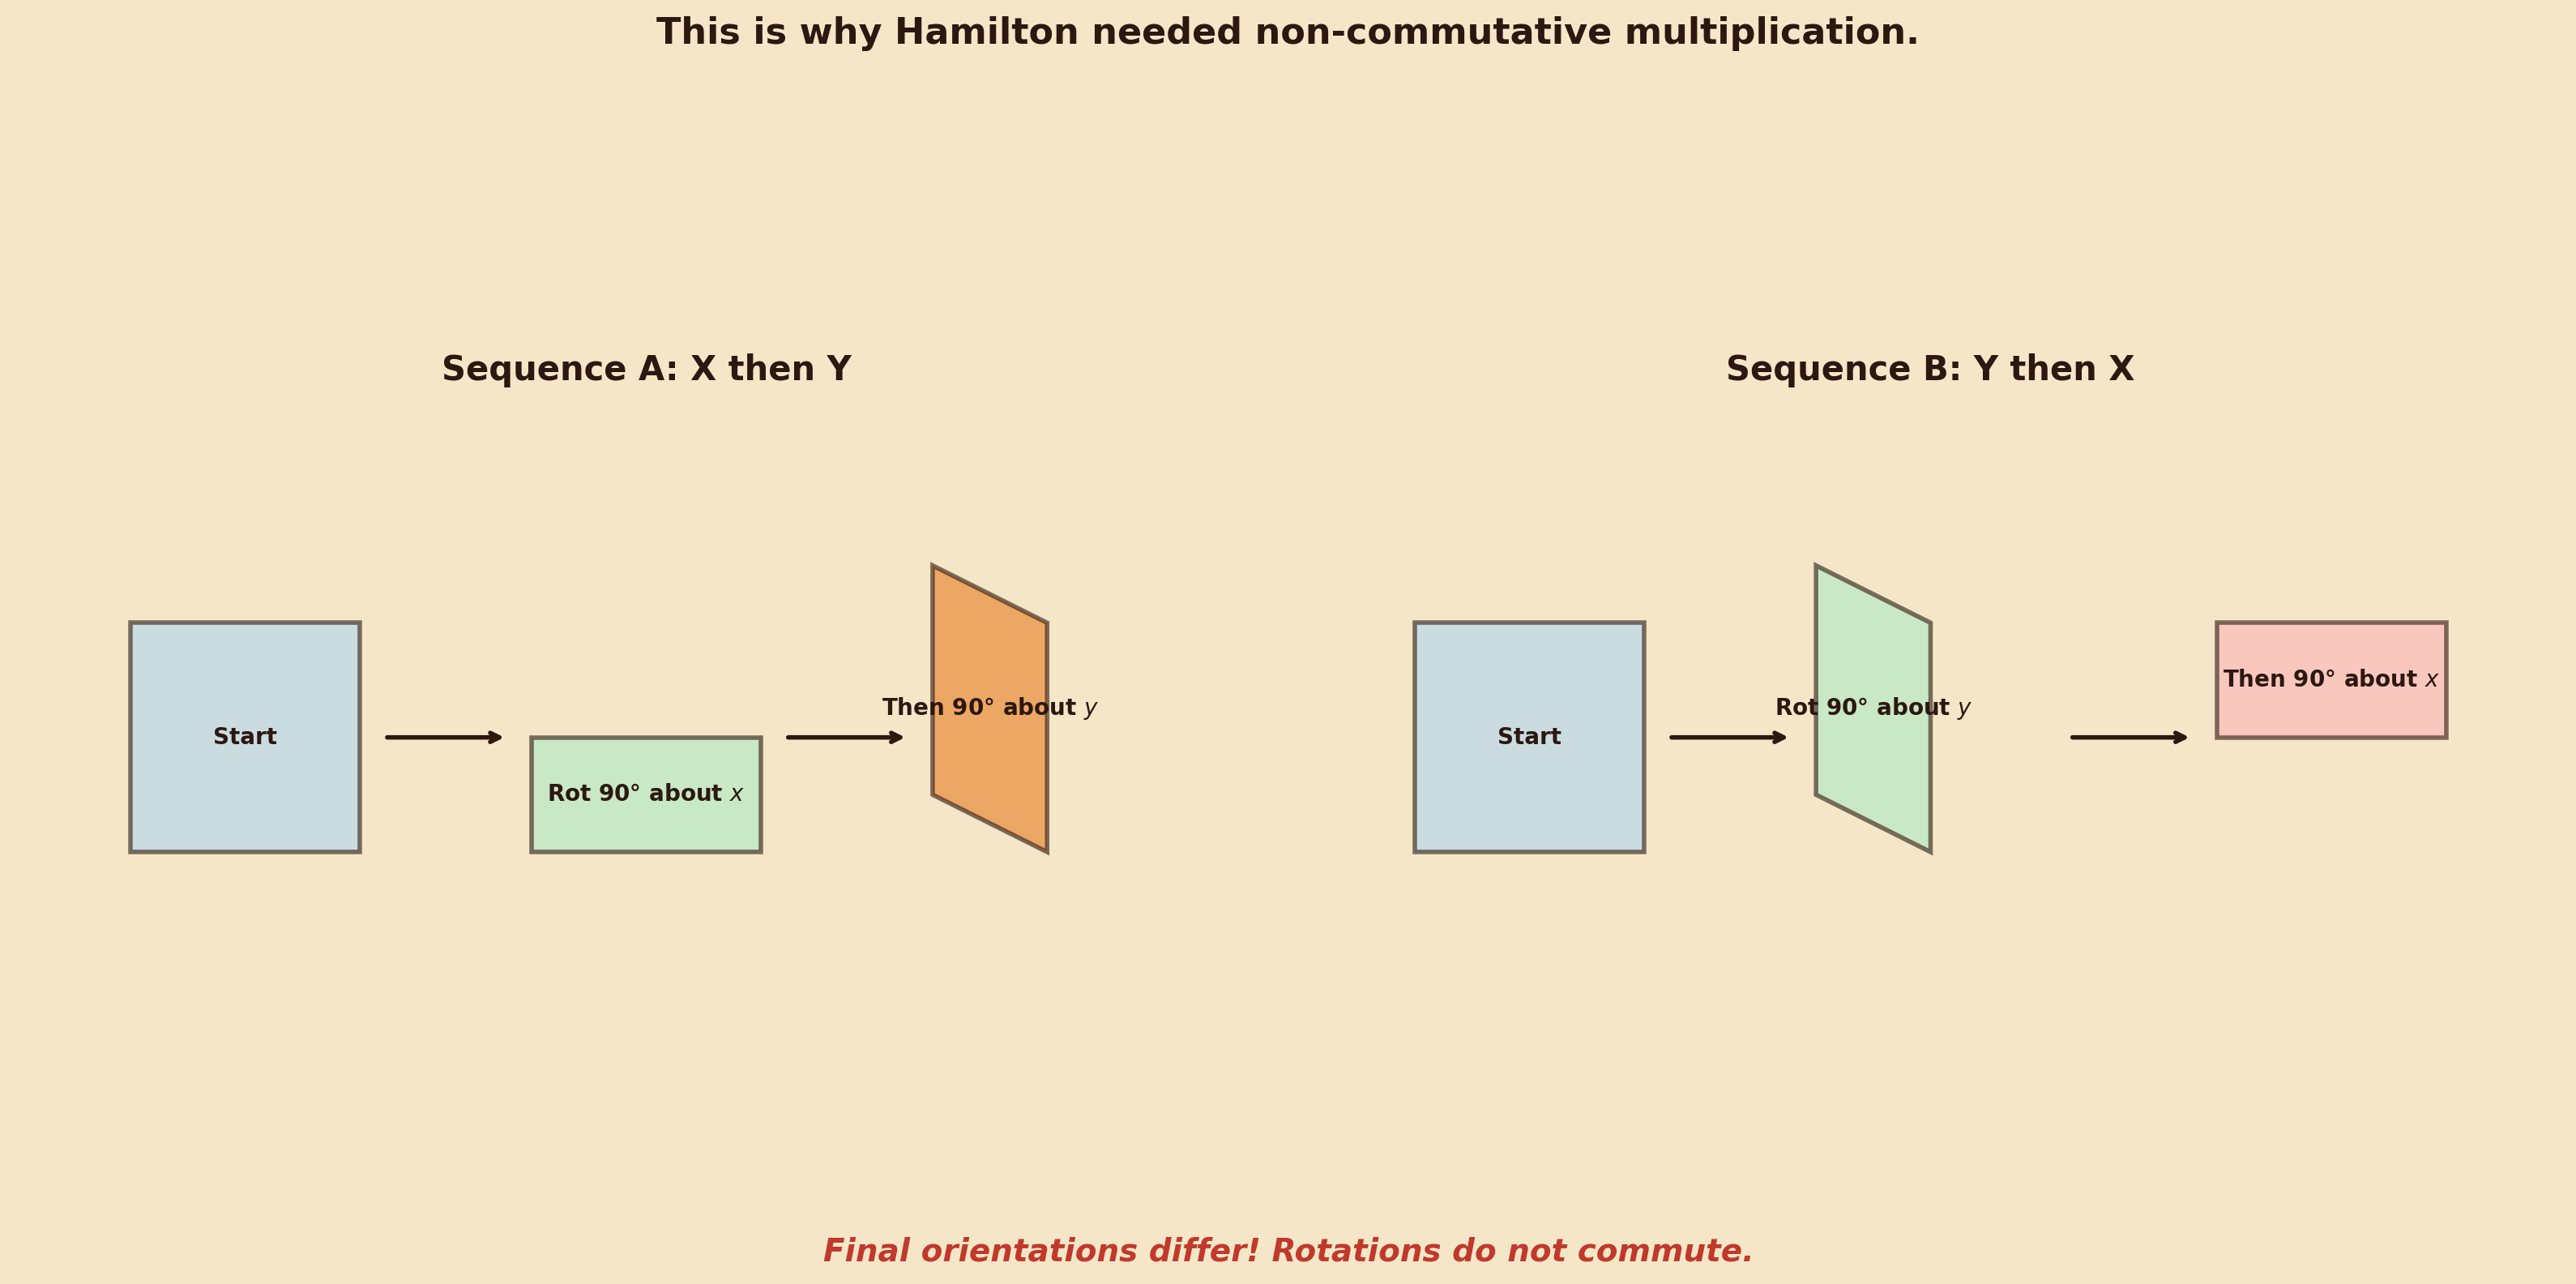
\includegraphics[width=0.82\textwidth,keepaspectratio]{images/chapter9_fig06_rotation_demo.png}
\caption{A physical demonstration of non-commutative rotation.}
\end{figure}


Three-dimensional rotations do not commute. Any algebra that faithfully represents them must therefore be non-commutative. Hamilton's quaternions\index{quaternions} are the \textit{minimal} such algebra --- the price of capturing the geometry of three-dimensional space is precisely the death of $ab = ba$. It is a stiff price, but the quaternions have paid dividends for nearly two centuries: they are the standard tool for encoding rotations in computer graphics, aerospace engineering, and robotics, precisely because they avoid the singularities ("gimbal lock") that plague other representations.


\ornbreak



\section{Euler's Grand Engine --- The Four-Square Identity}


The Brahmagupta–Fibonacci identity was a delightful trick for sums of \textit{two} squares. But Euler, being Euler, wanted more. In a 1748 letter to Goldbach, he posed the question: if two numbers are each a sum of four squares, is their product also a sum of four squares? And could one write down an explicit formula, analogous to Brahmagupta's, giving the four output squares in terms of the eight input values?

He found the answer was yes --- but the formula was a monster:

\textbf{Theorem (Euler's Four-Square Identity).}

\[
(x_1^2 + x_2^2 + x_3^2 + x_4^2)(y_1^2 + y_2^2 + y_3^2 + y_4^2)
\]

\[
= (x_1 y_1 - x_2 y_2 - x_3 y_3 - x_4 y_4)^2
\]

\[
+ (x_1 y_2 + x_2 y_1 + x_3 y_4 - x_4 y_3)^2
\]

\[
+ (x_1 y_3 - x_2 y_4 + x_3 y_1 + x_4 y_2)^2
\]

\[
+ (x_1 y_4 + x_2 y_3 - x_3 y_2 + x_4 y_1)^2.
\]

Look at the four output expressions on the right. Each involves all eight input variables, with a pattern of plus and minus signs that seems almost perverse in its complexity. Where Brahmagupta's identity was an elegant couplet, Euler's is a sprawling quartet. Yet the proof is the same brute-force verification: expand every square on the right, collect terms, watch the cross-terms cancel in pairs, and see that what remains is the product on the left.

\begin{figure}[htbp]
\centering
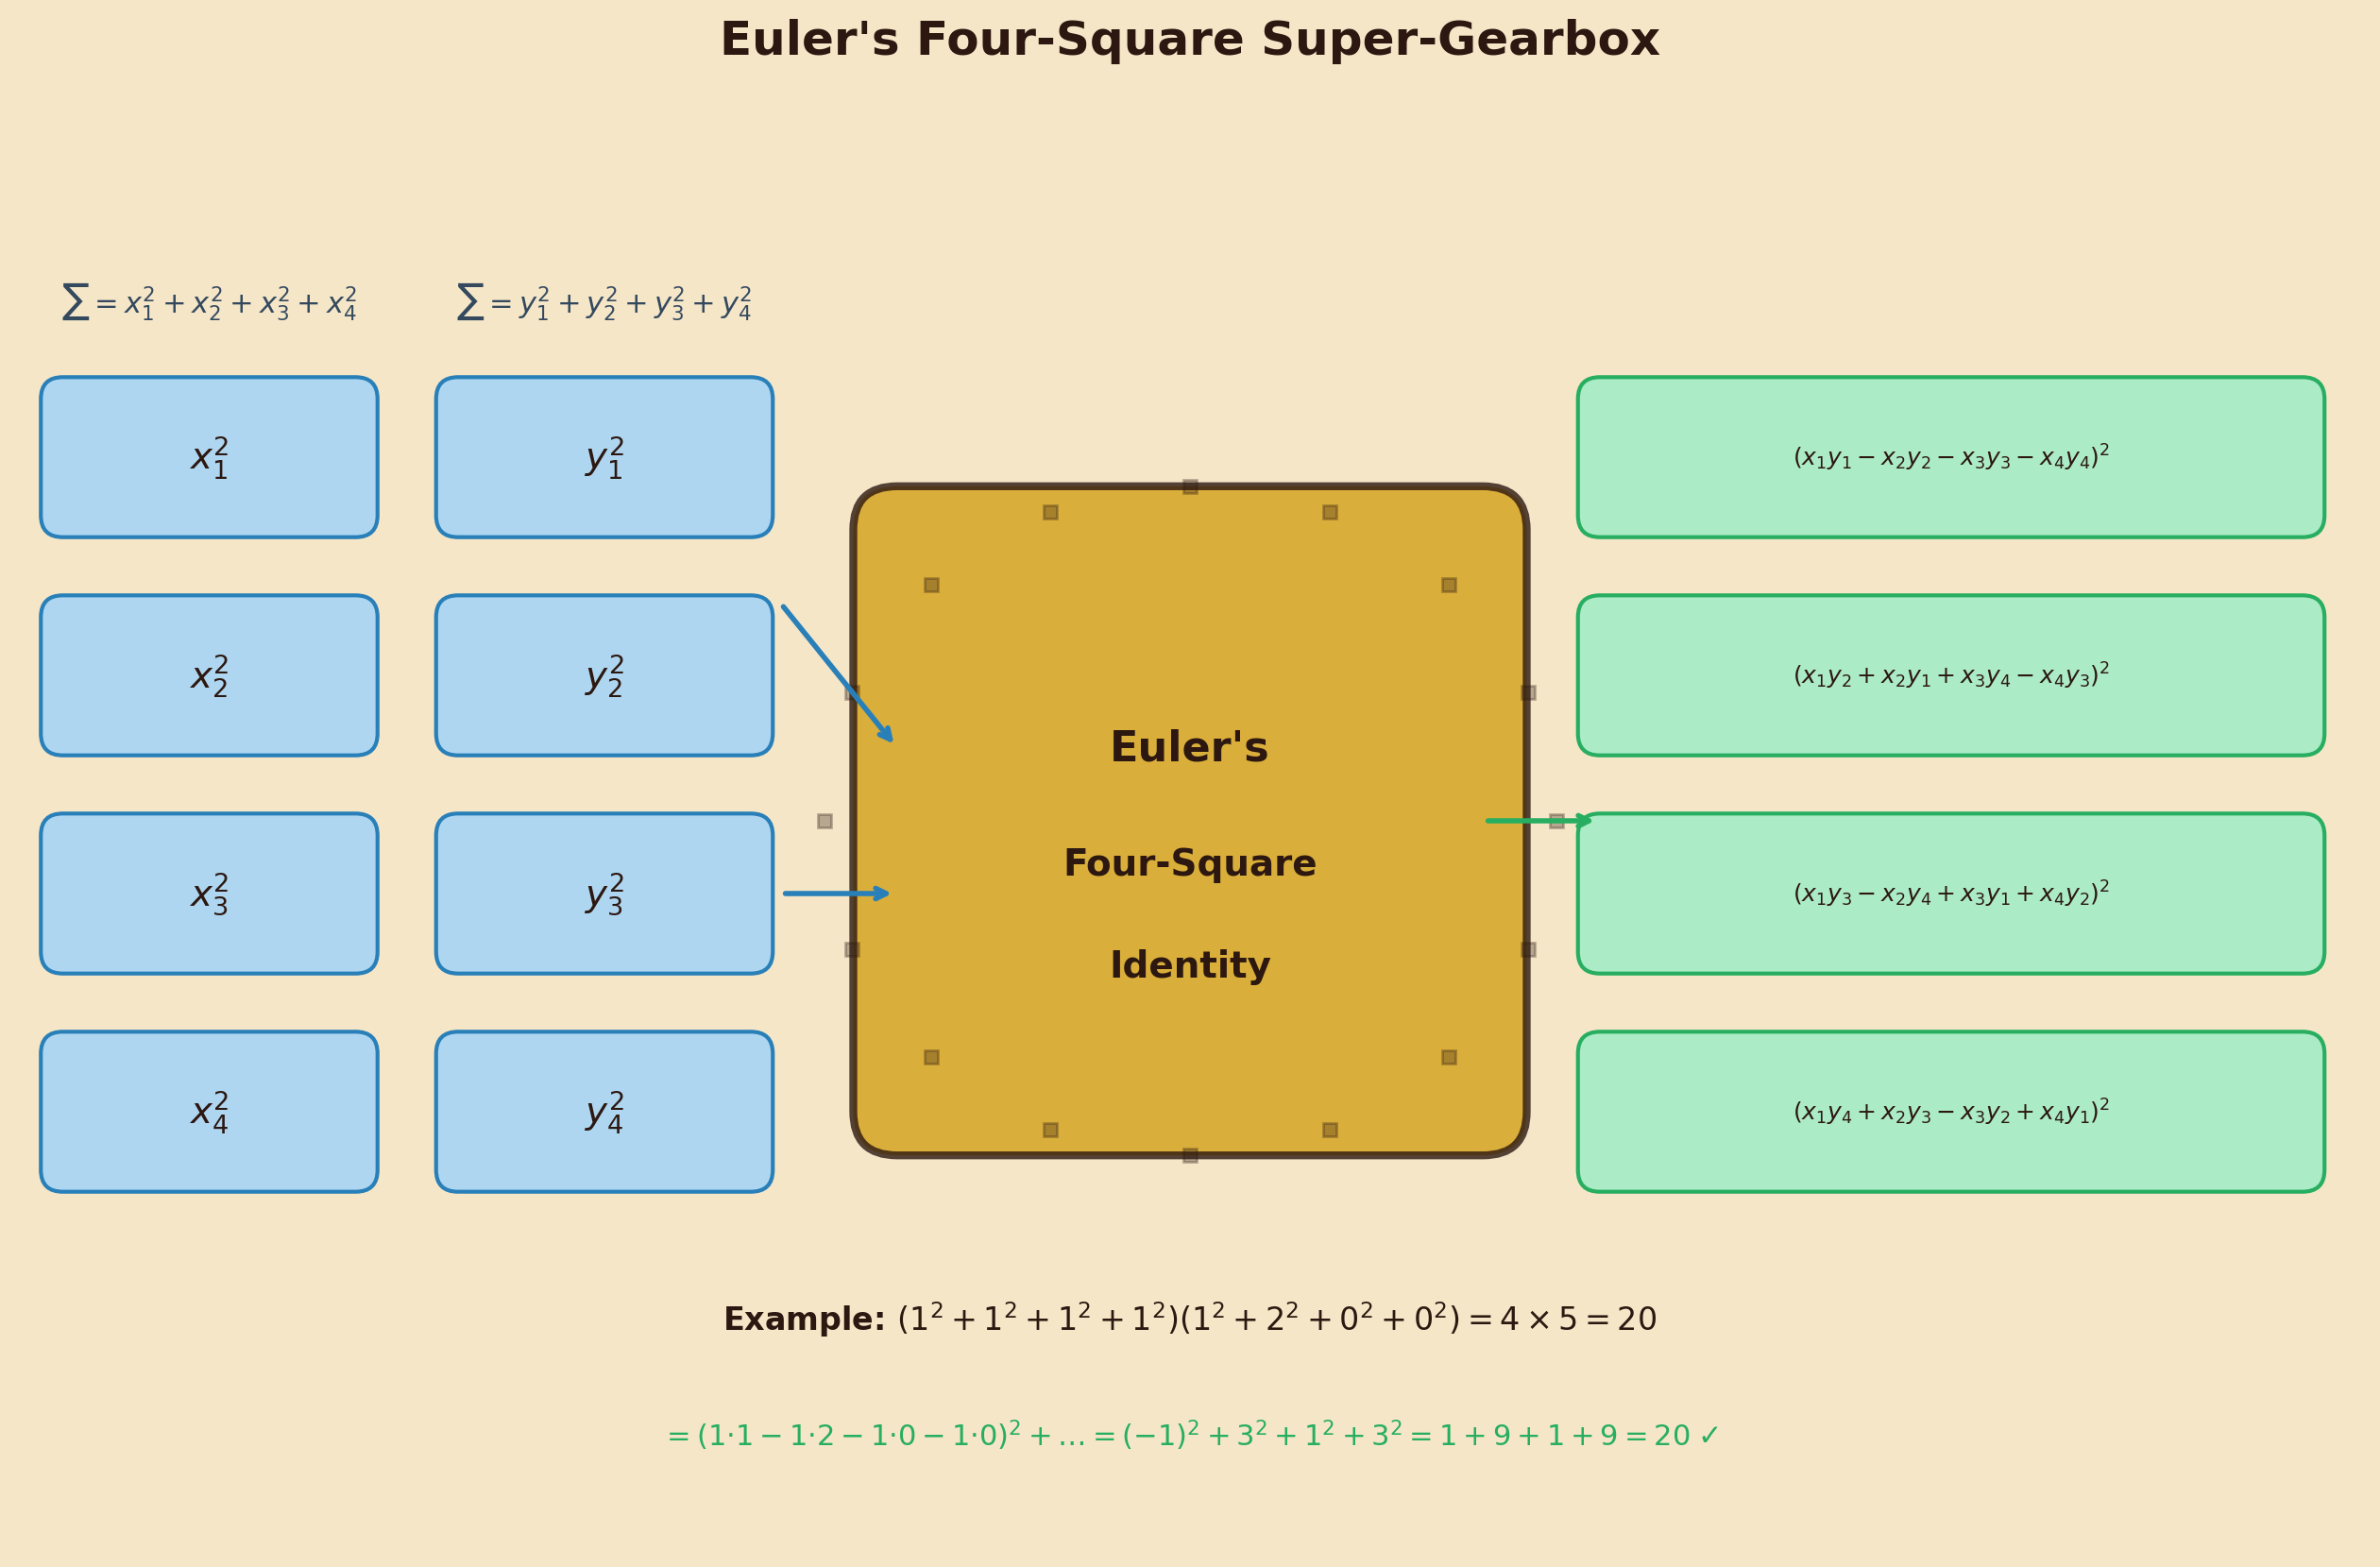
\includegraphics[width=0.82\textwidth,keepaspectratio]{images/chapter9_fig07_euler_gearbox.png}
\caption{A "super-gearbox" diagram similar to the Brahmagupta machine in Section 3, but now with four input slots on each side and four output slots.}
\end{figure}


But here is the revelation that Hamilton's quaternions provide. Define two quaternions:

\[
p = x_1 + x_2\mathbf{i} + x_3\mathbf{j} + x_4\mathbf{k}, \qquad q = y_1 + y_2\mathbf{i} + y_3\mathbf{j} + y_4\mathbf{k}.
\]

The quaternion norm-squared is $|p|^2 = x_1^2 + x_2^2 + x_3^2 + x_4^2$, and similarly for $q$. Now compute the product $p \cdot q$ using the quaternion multiplication rules. The four components of $p \cdot q$ are \textit{exactly} the four expressions inside the squares on the right side of Euler's identity. The entire monstrous formula is nothing but the statement:

\[
|p \cdot q|^2 = |p|^2 \cdot |q|^2.
\]

The quaternion norm is multiplicative --- just as the complex norm was. Euler's four-square identity, which he discovered by heroic algebraic computation, is simply the norm-multiplicativity of Hamilton's quaternions, which would not be discovered for another ninety-five years. Euler had found the shadow of a structure he could not yet see.

\begin{figure}[htbp]
\centering
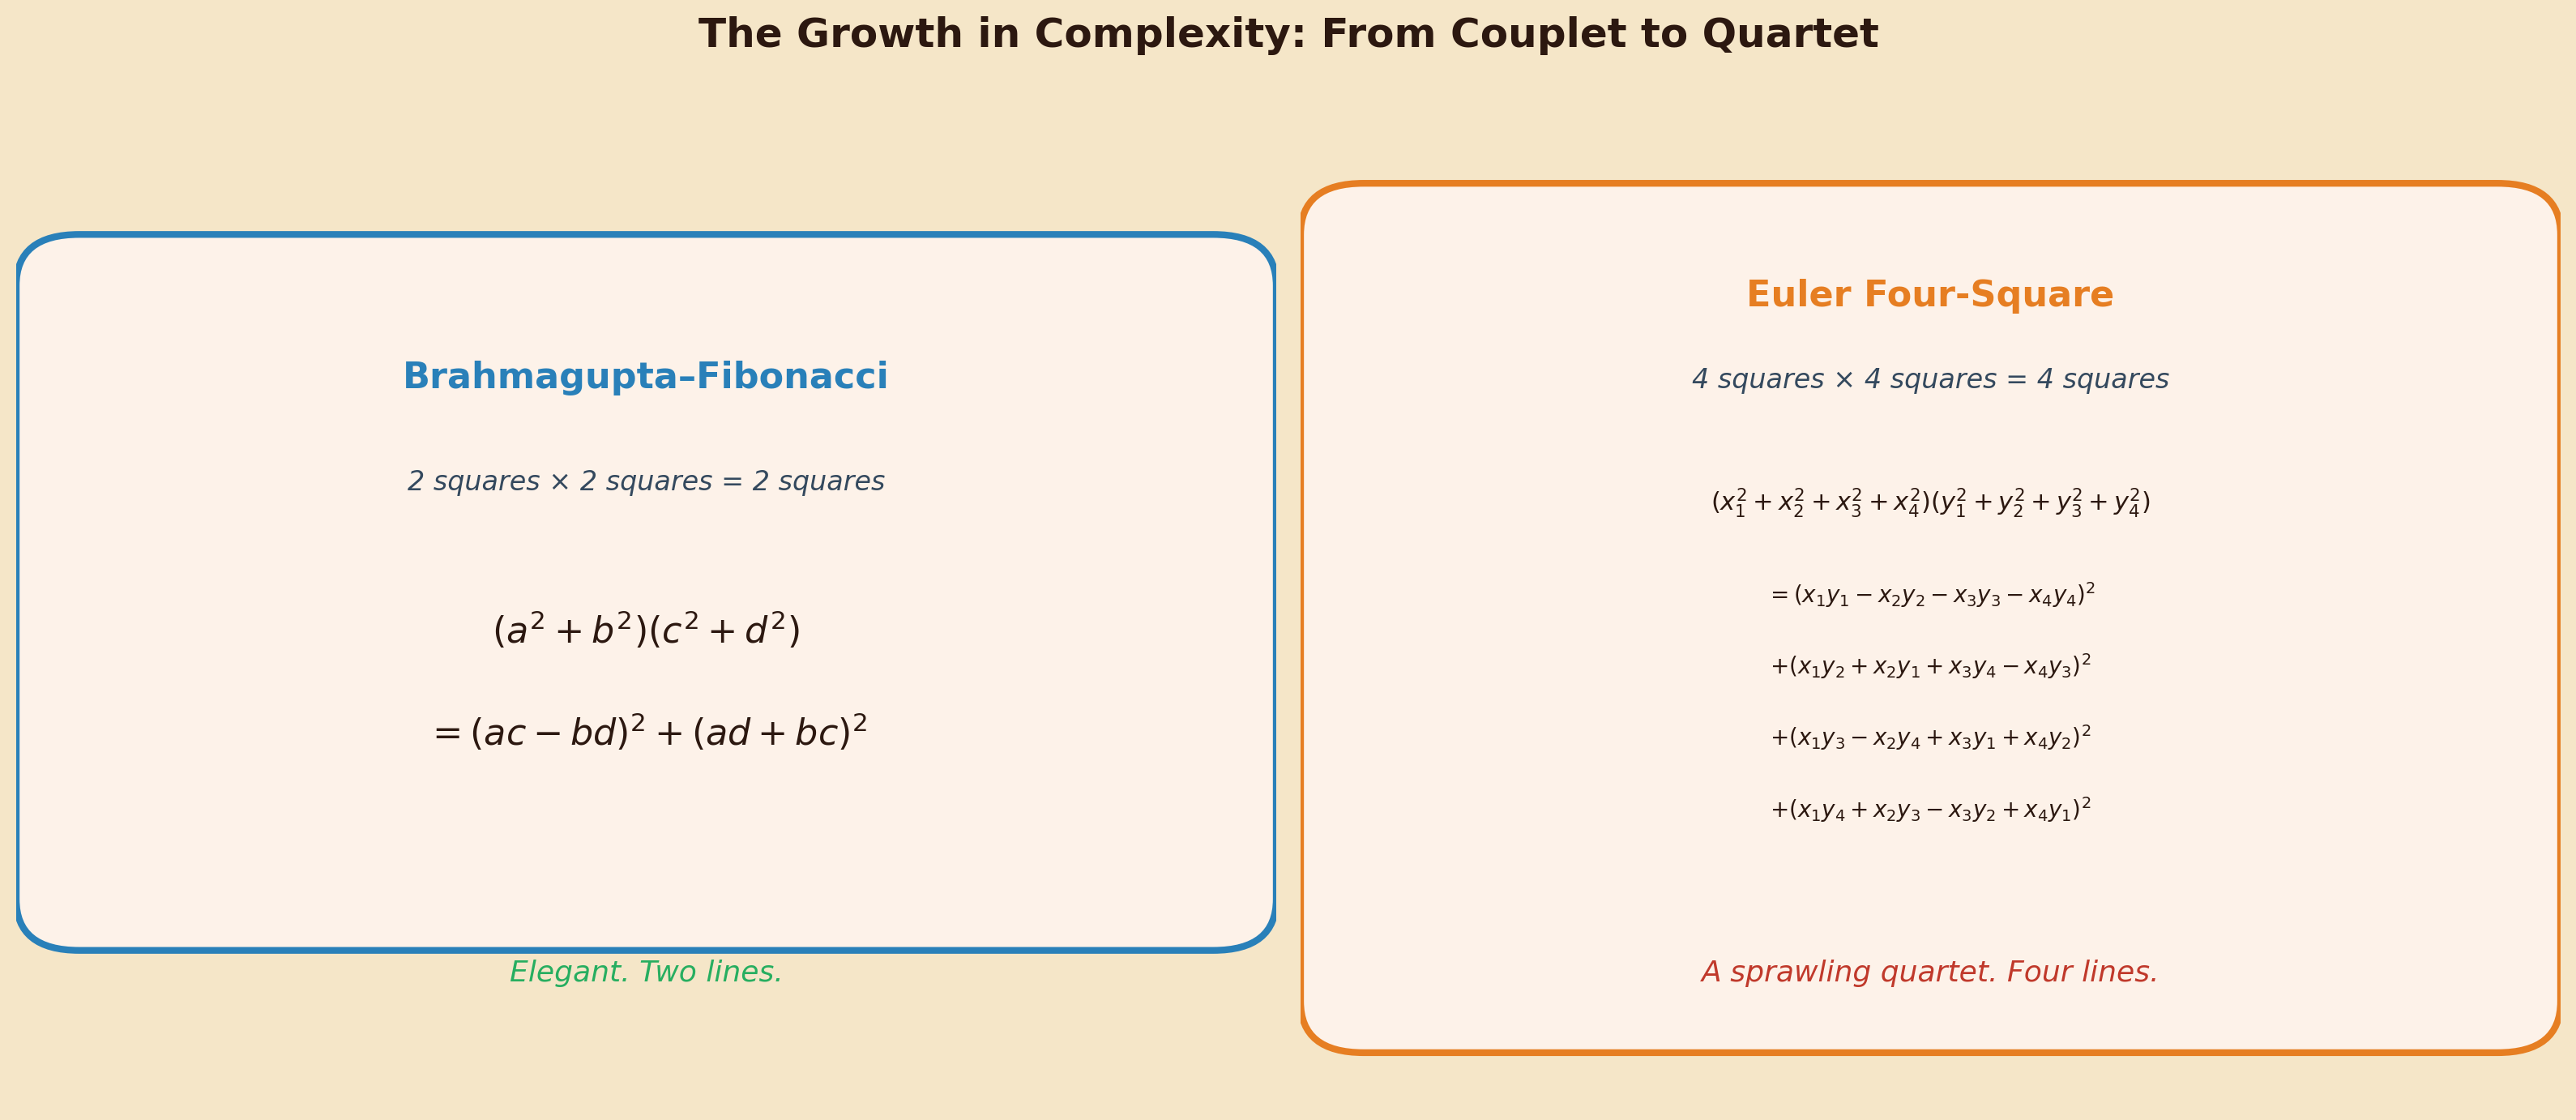
\includegraphics[width=0.82\textwidth,keepaspectratio]{images/chapter9_fig08_identity_comparison.png}
\caption{A side-by-side comparison table.}
\end{figure}


This identity was the key stepping stone toward one of the jewels of number theory: Lagrange's Four-Square Theorem, which asserts that \textit{every} positive integer can be written as a sum of four squares. Euler's identity reduces the problem to proving it for primes --- because if $m$ and $n$ are each sums of four squares, the identity guarantees that $mn$ is too. Lagrange then "only" had to handle the prime case, which he settled in 1770.

And Hurwitz, a century after Hamilton, would prove that such composition identities exist \textit{only} in dimensions $1$, $2$, $4$, and $8$. But we are getting ahead of ourselves.


\ornbreak



\section{The Staircase of Squares --- How Channels Nest Inside One Another}


If someone tells you a number is a perfect square --- say $n = 49 = 7^2$ --- can you also write it as a sum of two squares? Of course: $49 = 7^2 + 0^2$. Just append a zero. What about four squares? Easy: $49 = 7^2 + 0^2 + 0^2 + 0^2$. And eight? $49 = 7^2 + 0^2 + 0^2 + 0^2 + 0^2 + 0^2 + 0^2 + 0^2$.

This seems like cheating --- and in a sense it is. But what appears to be a trivial observation is actually the ground floor of a grand staircase that connects all four levels of the number tower.

\textbf{Step 1 $\to$ 2.} If $n = a^2$ (a sum of $1$ square), then $n = a^2 + 0^2$ (a sum of $2$ squares).

\textbf{Step 2 $\to$ 3.} If $n = a^2 + b^2$ (a sum of $2$ squares), then $n = a^2 + b^2 + 0^2 + 0^2$ (a sum of $4$ squares).

\textbf{Step 3 $\to$ 4.} If $n = a^2 + b^2 + c^2 + d^2$ (a sum of $4$ squares), then we can write:

\[
n = a^2 + b^2 + c^2 + d^2 + 0^2 + 0^2 + 0^2 + 0^2 = \sum_{i=0}^{7} f(i)^2,
\]

where $f(0) = a$, $f(1) = b$, $f(2) = c$, $f(3) = d$, and $f(4) = f(5) = f(6) = f(7) = 0$.

\begin{figure}[htbp]
\centering
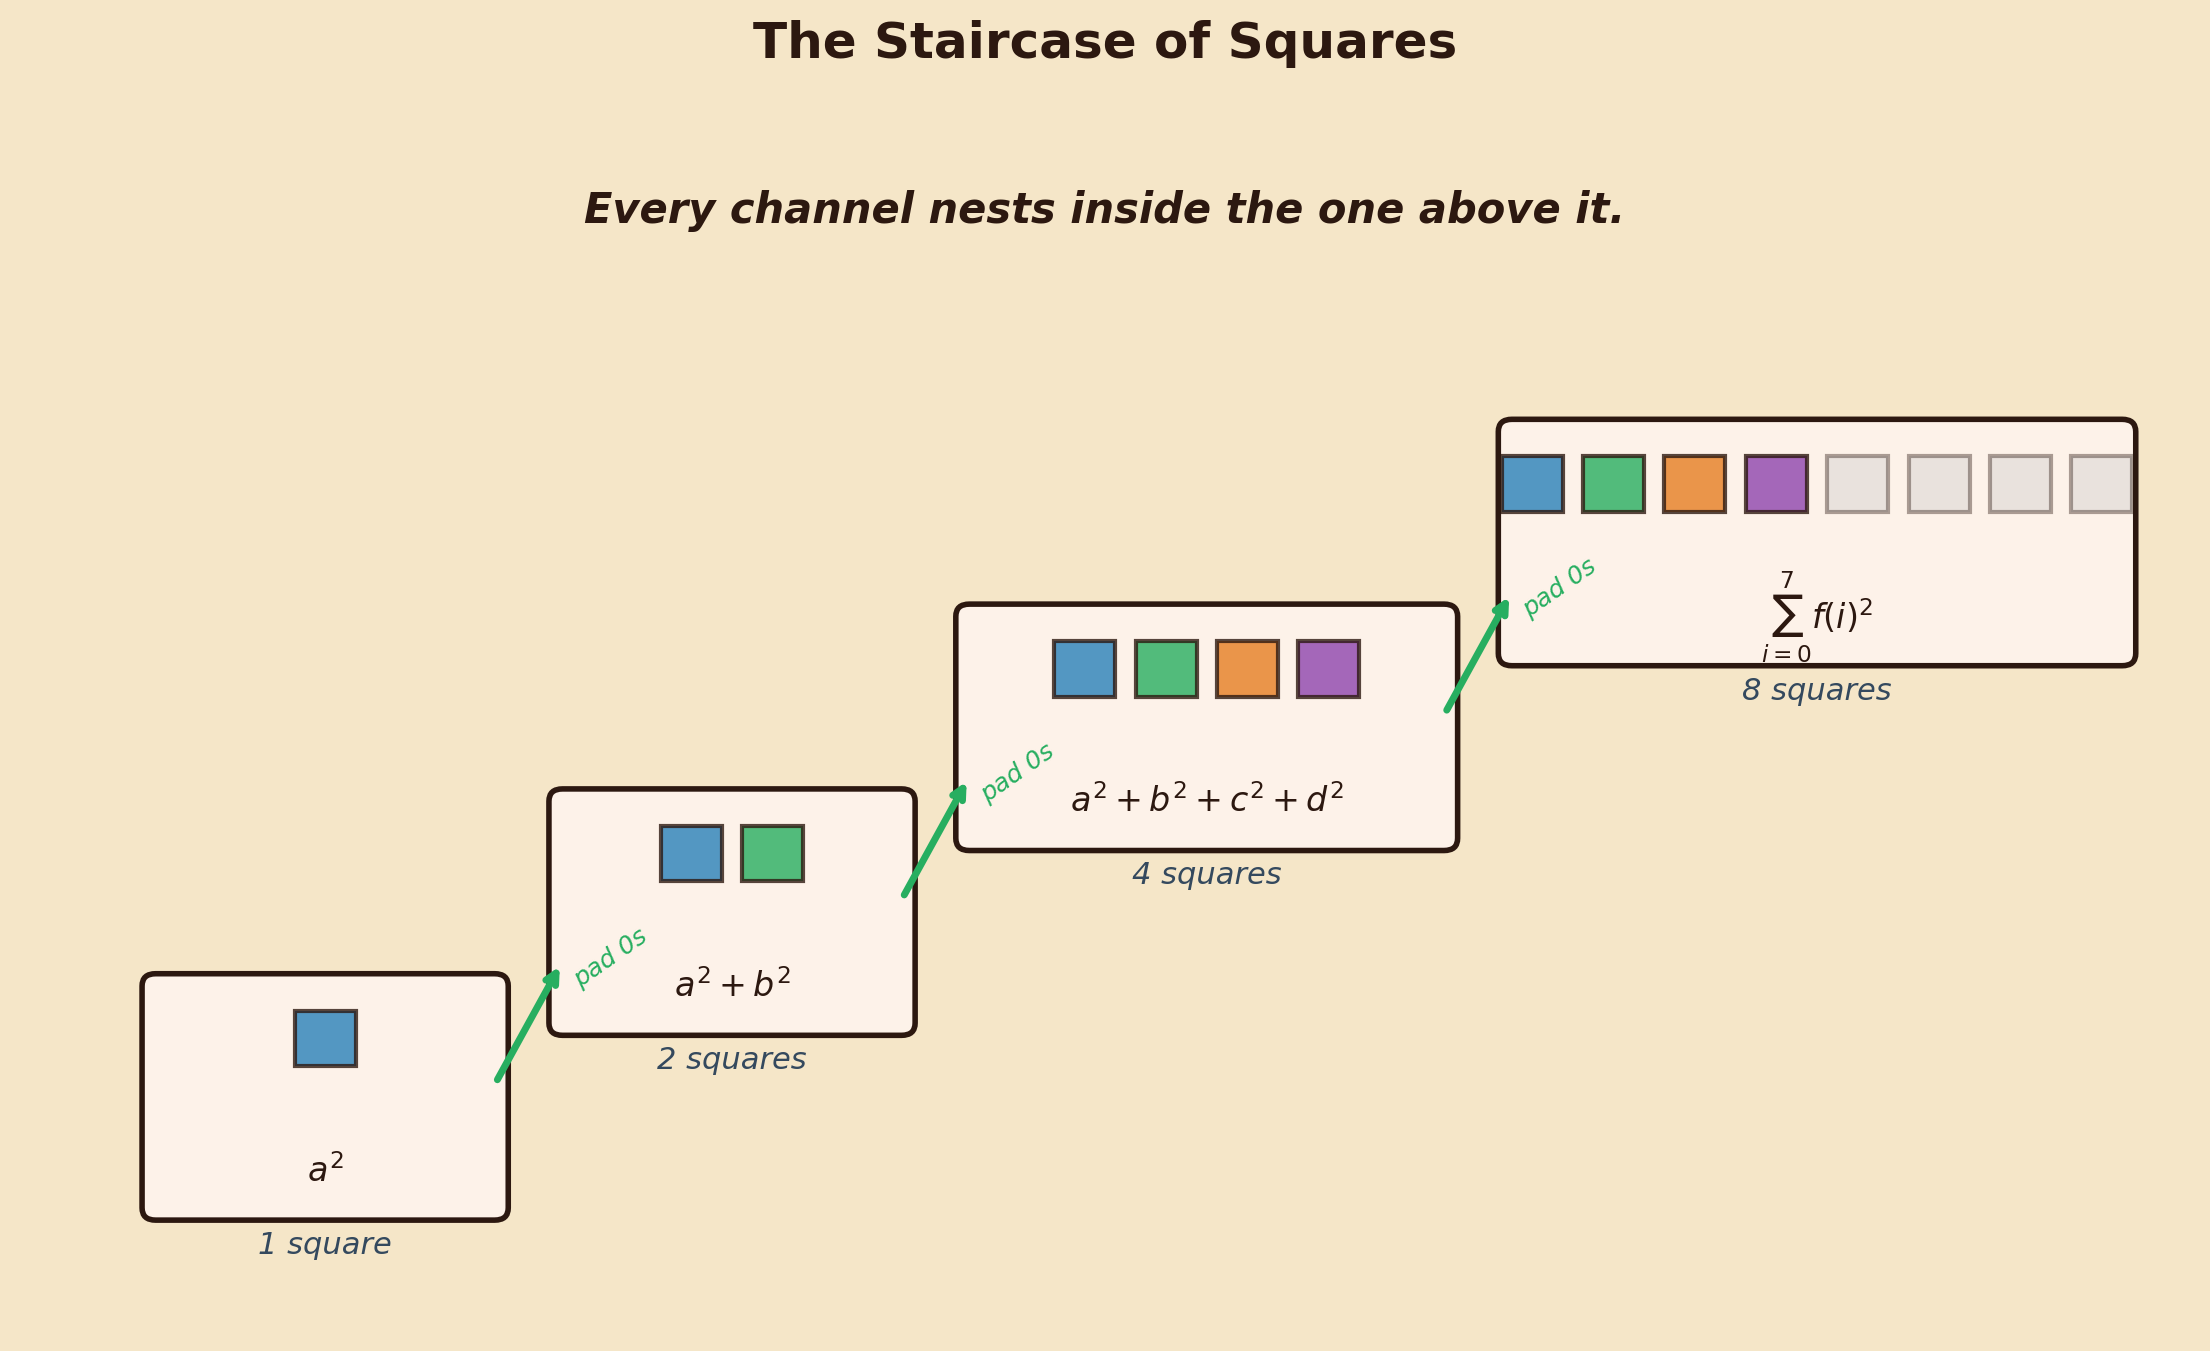
\includegraphics[width=0.82\textwidth,keepaspectratio]{images/chapter9_fig09_staircase.png}
\caption{A staircase with four steps, ascending from left to right.}
\end{figure}


The proof in each case is the same padding argument: extend the representation with zeros. But the conceptual meaning runs deeper. The set of integers representable as a sum of $1$ square is \textit{contained} in the set representable as a sum of $2$ squares, which is contained in the set of $4$ squares, which is contained in the set of $8$ squares. Every channel nests inside the one above it like a series of Russian dolls. The higher you climb on the ladder, the more numbers you can represent --- until, at level four (sums of four squares), you already capture every positive integer by Lagrange's theorem.

The padding argument also tells us something about the \textit{composition identities}. Since $\mathbb{R} \subset \mathbb{C} \subset \mathbb{H} \subset \mathbb{O}$ (each algebra embeds in the next), the Brahmagupta identity is a "special case" of Euler's four-square identity (set $x_3 = x_4 = y_3 = y_4 = 0$), which is in turn a special case of the eight-square identity for octonions. The staircase of embeddings generates a staircase of identities, each more powerful --- and more complex --- than the one below.


\ornbreak



\section{The Magic Dimensions --- Why $1, 2, 4, 8$ and Nothing Else}


Here is a list of numbers: $1, 2, 4, 8$. What do they have in common? Any child will say, "They're powers of two!" And indeed:

\[
1 = 2^0, \quad 2 = 2^1, \quad 4 = 2^2, \quad 8 = 2^3.
\]

But these particular powers of two are special in a way that $16$, $32$, $64$, and all subsequent powers are not. In these dimensions, and \textit{only} these dimensions, can you build a number system where the norm is multiplicative --- a \textit{composition algebra}, a system where:

\[
|x \cdot y| = |x| \cdot |y|
\]

for all elements $x$ and $y$. After dimension $8$, the ladder breaks. No amount of cleverness, no rearrangement of signs, no alternative multiplication rule can rescue the multiplicativity of the norm in dimension $16$ or beyond.

This was proved by Adolf Hurwitz\index{Hurwitz, Adolf}\index{Hurwitz theorem} in 1898:

\textbf{Theorem (Hurwitz, 1898).} *A normed division algebra over $\mathbb{R}$ must have dimension $1$, $2$, $4$, or $8$.*

\begin{figure}[htbp]
\centering
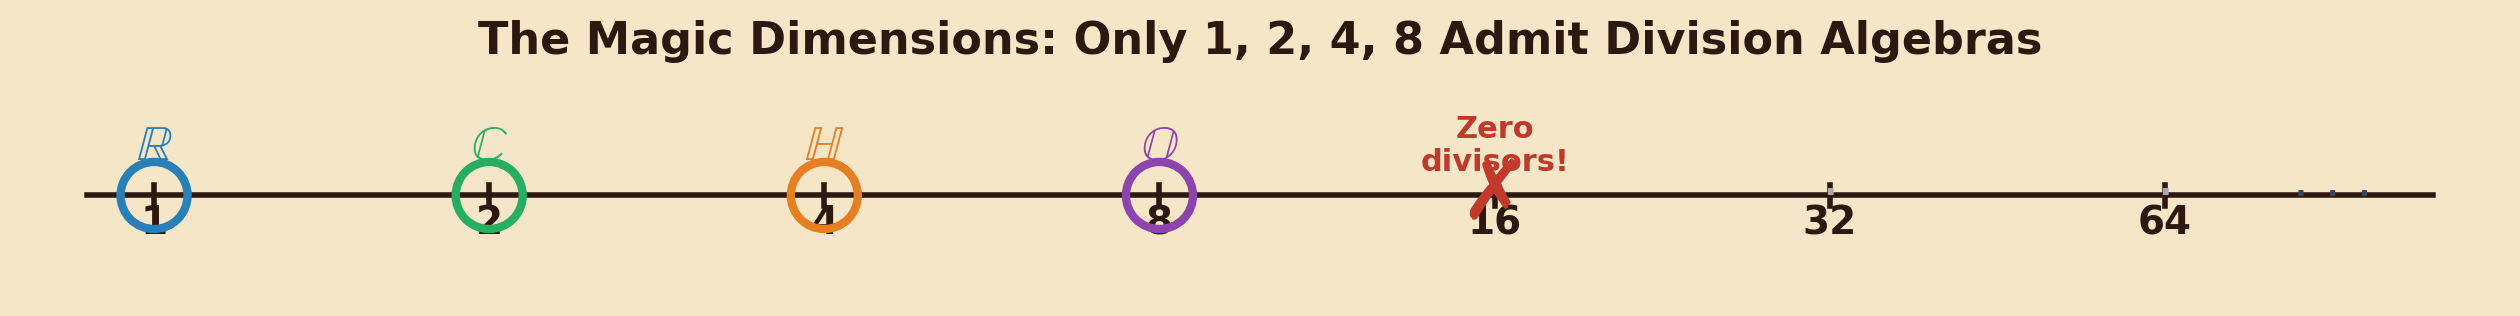
\includegraphics[width=0.82\textwidth,keepaspectratio]{images/chapter9_fig10_magic_dimensions.png}
\caption{A number line showing powers of $2$: $1, 2, 4, 8, 16, 32, \ldots$ The first four are circled and labeled $\mathbb{R}, \mathbb{C}, \mathbb{H}, \mathbb{O}$.}
\end{figure}


Why does $16$ fail? The sedenions $\mathbb{S}$ contain explicit zero divisors. Here is one: define

\[
e = (e_1 + e_{10}) \quad \text{and} \quad f = (e_2 + e_{11}),
\]

where $e_1, e_2, e_{10}, e_{11}$ are certain basis elements of $\mathbb{S}$. Then $e \neq 0$ and $f \neq 0$, yet $e \cdot f = 0$. The norm cannot be multiplicative in such a system, because $|e| \cdot |f| > 0$ while $|e \cdot f| = |0| = 0$.

The numerical coincidences are irresistible. The sum $1 + 2 + 4 + 8 = 15 = 2^4 - 1$ is a Mersenne number (though not a Mersenne prime). The product $1 \times 2 \times 4 \times 8 = 64 = 2^6$. The sequence $0, 1, 2, 3$ of exponents is itself the simplest possible arithmetic progression. Whether these numerological patterns are meaningful or merely decorative is a question that mathematicians have debated, inconclusively, for over a century.

\begin{figure}[htbp]
\centering
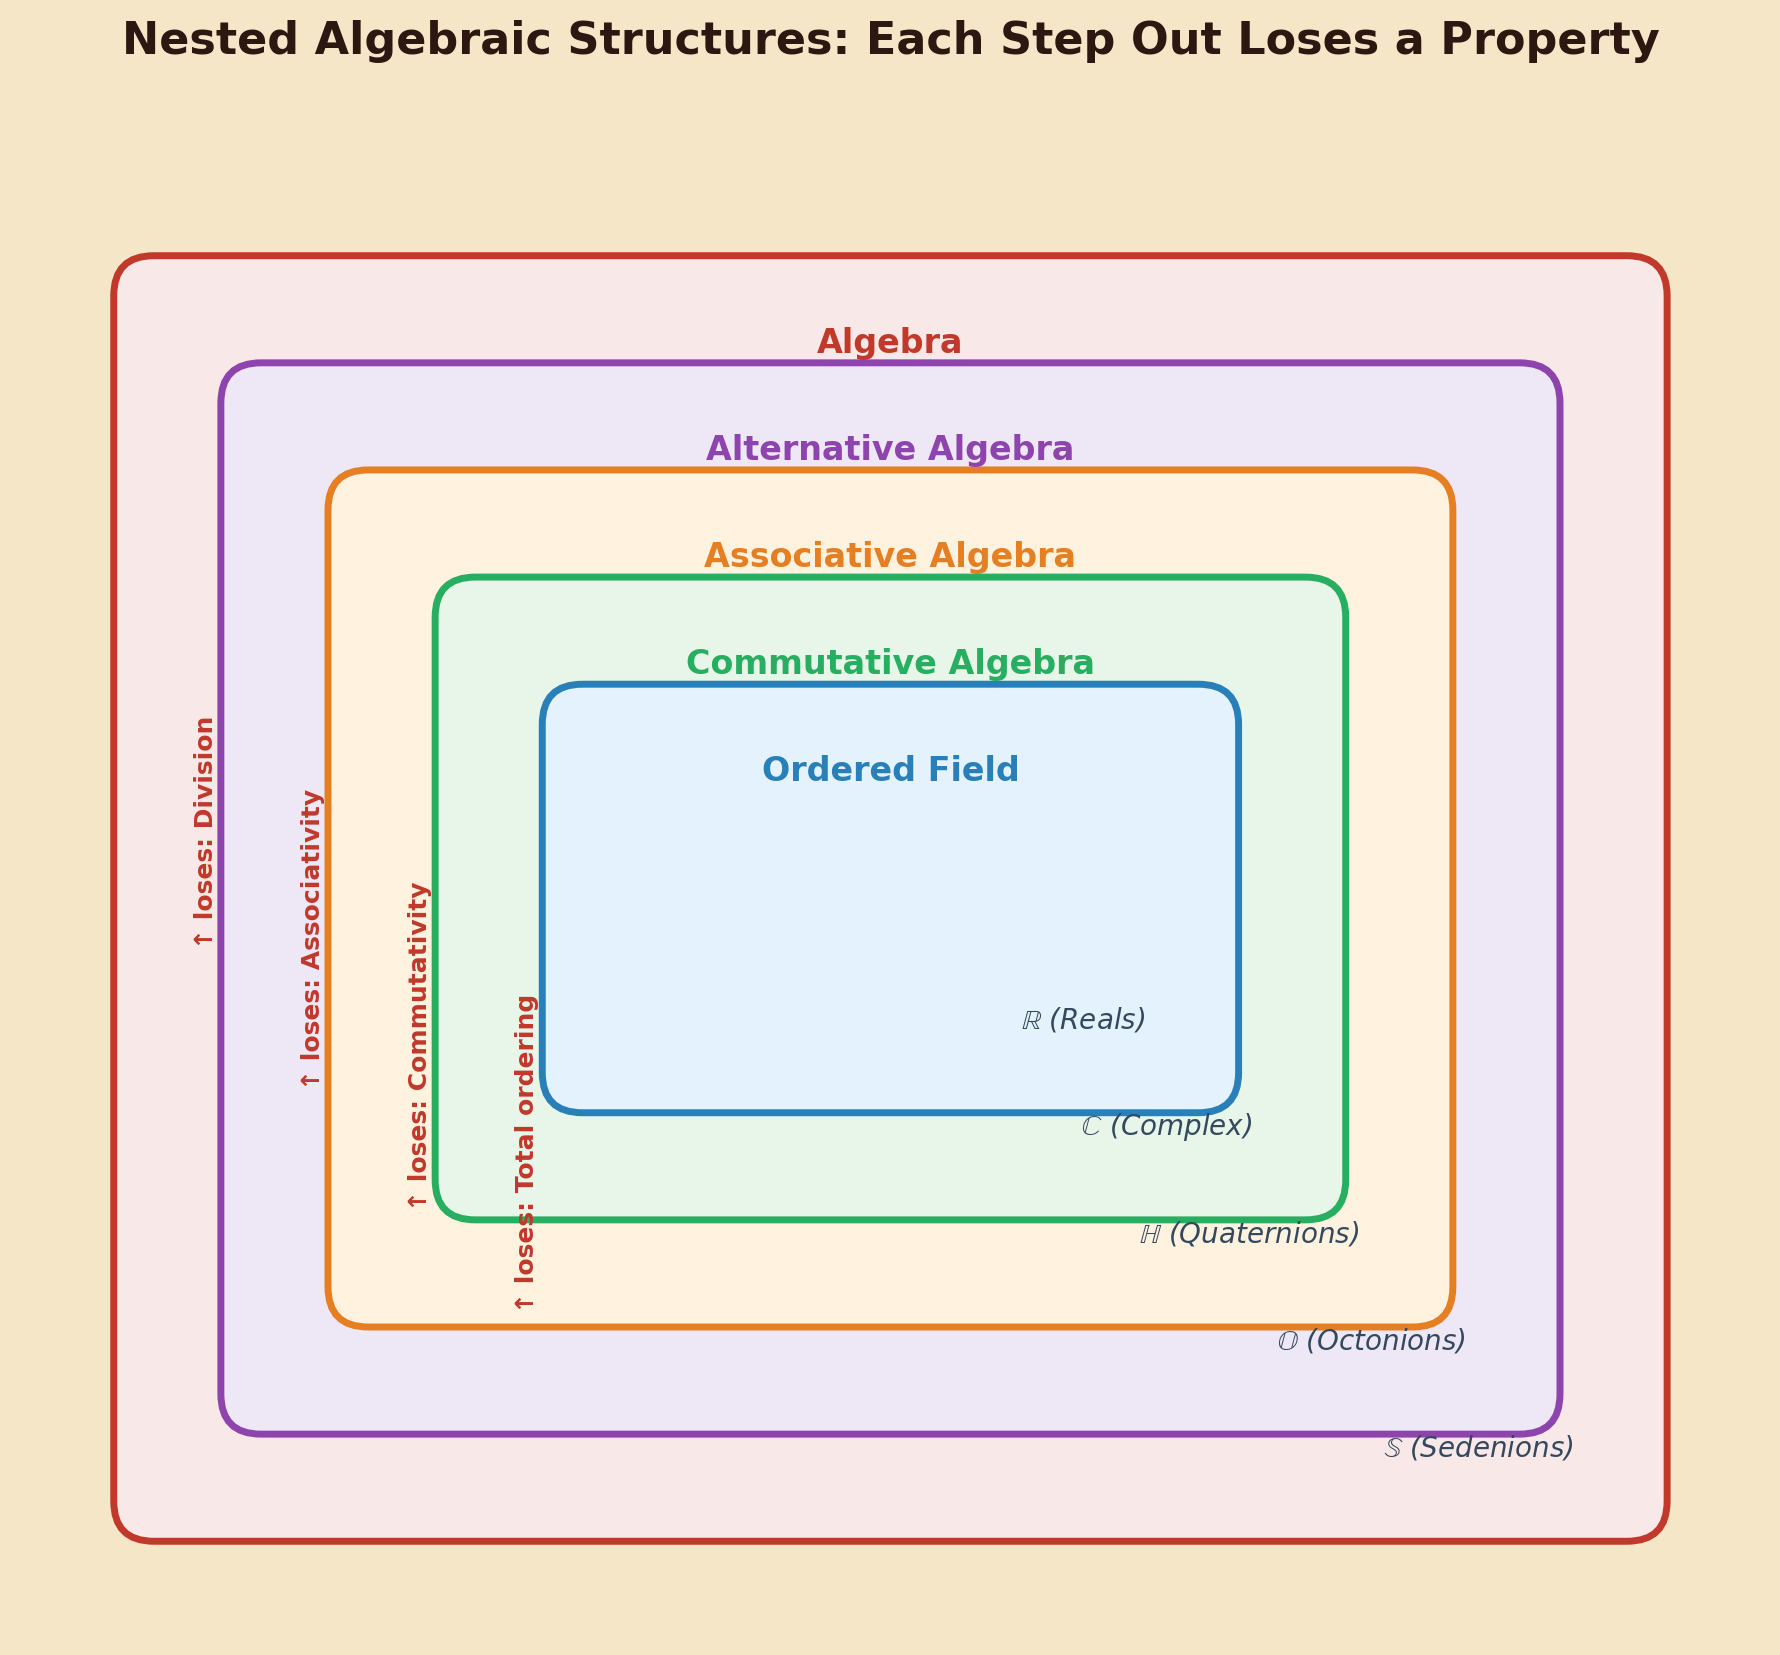
\includegraphics[width=0.82\textwidth,keepaspectratio]{images/chapter9_fig11_venn_algebras.png}
\caption{A Venn diagram of algebraic properties.}
\end{figure}


The deeper story involves topology. In 1958, Raoul Bott proved his famous periodicity theorem, which shows that the homotopy groups of the classical groups repeat with period $8$ --- a phenomenon now called \textit{Bott periodicity}. The four normed division algebras sit at the four "corners" of this period-$8$ cycle, and their existence is intimately tied to the topology of spheres: the only spheres that are parallelizable (that is, that admit a global field of tangent frames) are $S^0$, $S^1$, $S^3$, and $S^7$ --- of dimensions $0$, $1$, $3$, and $7$, which are one less than the magic numbers $1$, $2$, $4$, $8$. The coincidences run so deep that John Baez, in his celebrated survey article on the octonions, called them "not just a pun but a theorem."


\ornbreak



\section{Guarding the Gate --- How Many Ways Can a Number Be a Perfect Square?}


How many integers $a$ satisfy $a^2 = 25$? Easy: $a = 5$ and $a = -5$. That is two. What about $a^2 = 7$? None (among the integers). Can it ever be more than two? What is the \textit{maximum} number of integer solutions to $a^2 = n$ for \textit{any} positive integer $n$?

The answer is exactly what you would guess: at most two.

\textbf{Theorem (Representation Bound for Squares).} *For any positive integer $n$, the number of integers $a$ with $|a| \leq n$ and $a^2 = n$ is at most $2$.*

The proof barely deserves the name. If $a^2 = n$, then $a = +\sqrt{n}$ or $a = -\sqrt{n}$. These are at most two values, and they are integers only when $n$ is a perfect square. In the "Channel 0" of our hierarchy --- where we represent a number by a single square --- the decoder has \textit{bandwidth} at most $2$. $\blacksquare$

\begin{figure}[htbp]
\centering
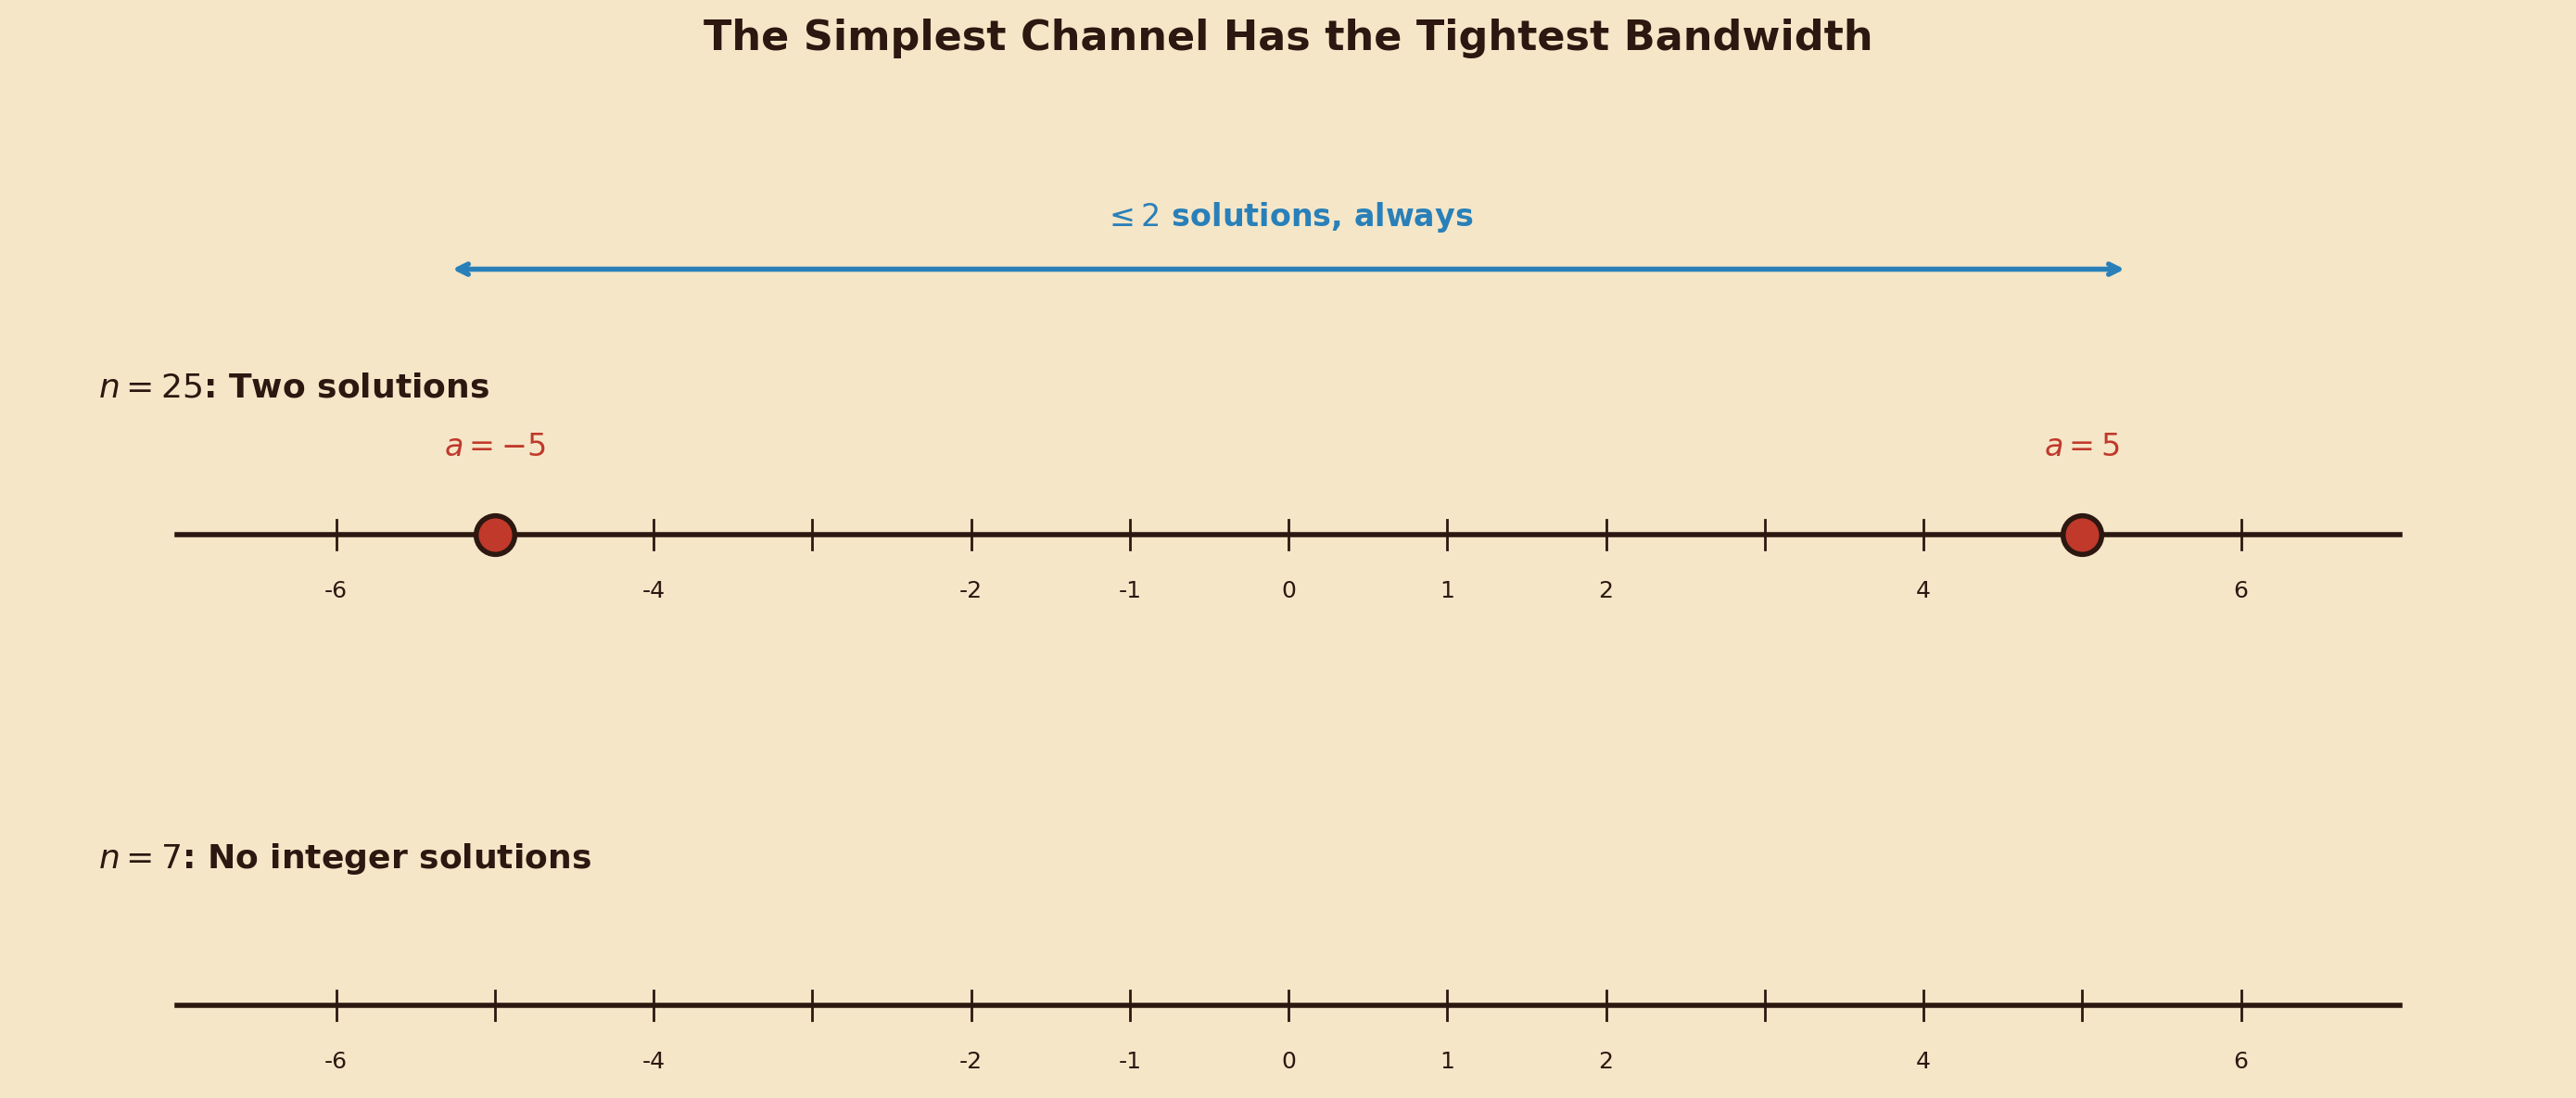
\includegraphics[width=0.82\textwidth,keepaspectratio]{images/chapter9_fig12_square_root_bandwidth.png}
\caption{A number line from $-25$ to $25$ with integer tick marks.}
\end{figure}


This tight bound stands in stark contrast to the higher channels. How many representations does $n$ have as a sum of two squares? The answer depends delicately on the prime factorization of $n$ and is governed by a theorem involving Dirichlet characters. How many representations as a sum of four squares? The answer is governed by a formula of stunning simplicity --- Jacobi\index{Jacobi, Carl Gustav Jacob}'s formula, to which we now turn.

The progression is clear: as the dimension of the channel grows, the number of representations explodes. Channel 0 permits at most $2$ representations. Channel 1 (sums of two squares) permits a number that grows with the divisor structure of $n$. Channel 2 (sums of four squares) permits a count that is a simple multiple of a divisor sum. The higher you climb, the richer the arithmetic, but also the more information each representation encodes.


\ornbreak



\section{Jacobi's Magnificent Formula --- Counting Representations by Four Squares}


We have seen that every positive integer is a sum of four squares (Lagrange's theorem). But \textit{how many ways} can a number be so expressed? By "how many ways," we mean the number of ordered quadruples $(a, b, c, d) \in \mathbb{Z}^4$ with $a^2 + b^2 + c^2 + d^2 = n$, where different signs and different orderings count as different representations. This is the function $r_4(n)$, and computing it for even small $n$ is a surprisingly entertaining exercise.

Take $n = 1$. The equation $a^2 + b^2 + c^2 + d^2 = 1$ demands that exactly one of the four variables is $\pm 1$ and the other three are $0$. There are $4$ choices for which variable is nonzero, and $2$ choices of sign, giving $r_4(1) = 8$.

Take $n = 2$. Now we need two of the four variables to be $\pm 1$ and the other two to be $0$. There are $\binom{4}{2} = 6$ ways to choose which two are nonzero, and $2^2 = 4$ sign choices, giving $r_4(2) = 24$.

Take $n = 3$. We need three variables $\pm 1$ and one $0$: that is $\binom{4}{3} \times 2^3 = 32$ ways. So $r_4(3) = 32$.

Is there a pattern? In 1834, Carl Gustav Jacob Jacobi found one --- and it is breathtakingly simple.

First, define a function of $n$:

\[
J(n) = \sum_{\substack{d \mid n \\ 4 \nmid d}} d.
\]

That is, $J(n)$ is the sum of all divisors of $n$ that are \textit{not} divisible by $4$. For example:

\begin{itemize}[leftmargin=*]
\item The divisors of $1$ are $\{1\}$. None are divisible by $4$, so $J(1) = 1$.
\item The divisors of $5$ are $\{1, 5\}$. Neither is divisible by $4$, so $J(5) = 1 + 5 = 6$.
\item The divisors of $12$ are $\{1, 2, 3, 4, 6, 12\}$. Those divisible by $4$ are $\{4, 12\}$. The rest sum to $J(12) = 1 + 2 + 3 + 6 = 12$.
\end{itemize}

\textbf{Theorem (Jacobi's Four-Square Theorem).} *For every positive integer $n$,*

\[
r_4(n) = 8 \cdot J(n).
\]

\begin{figure}[htbp]
\centering
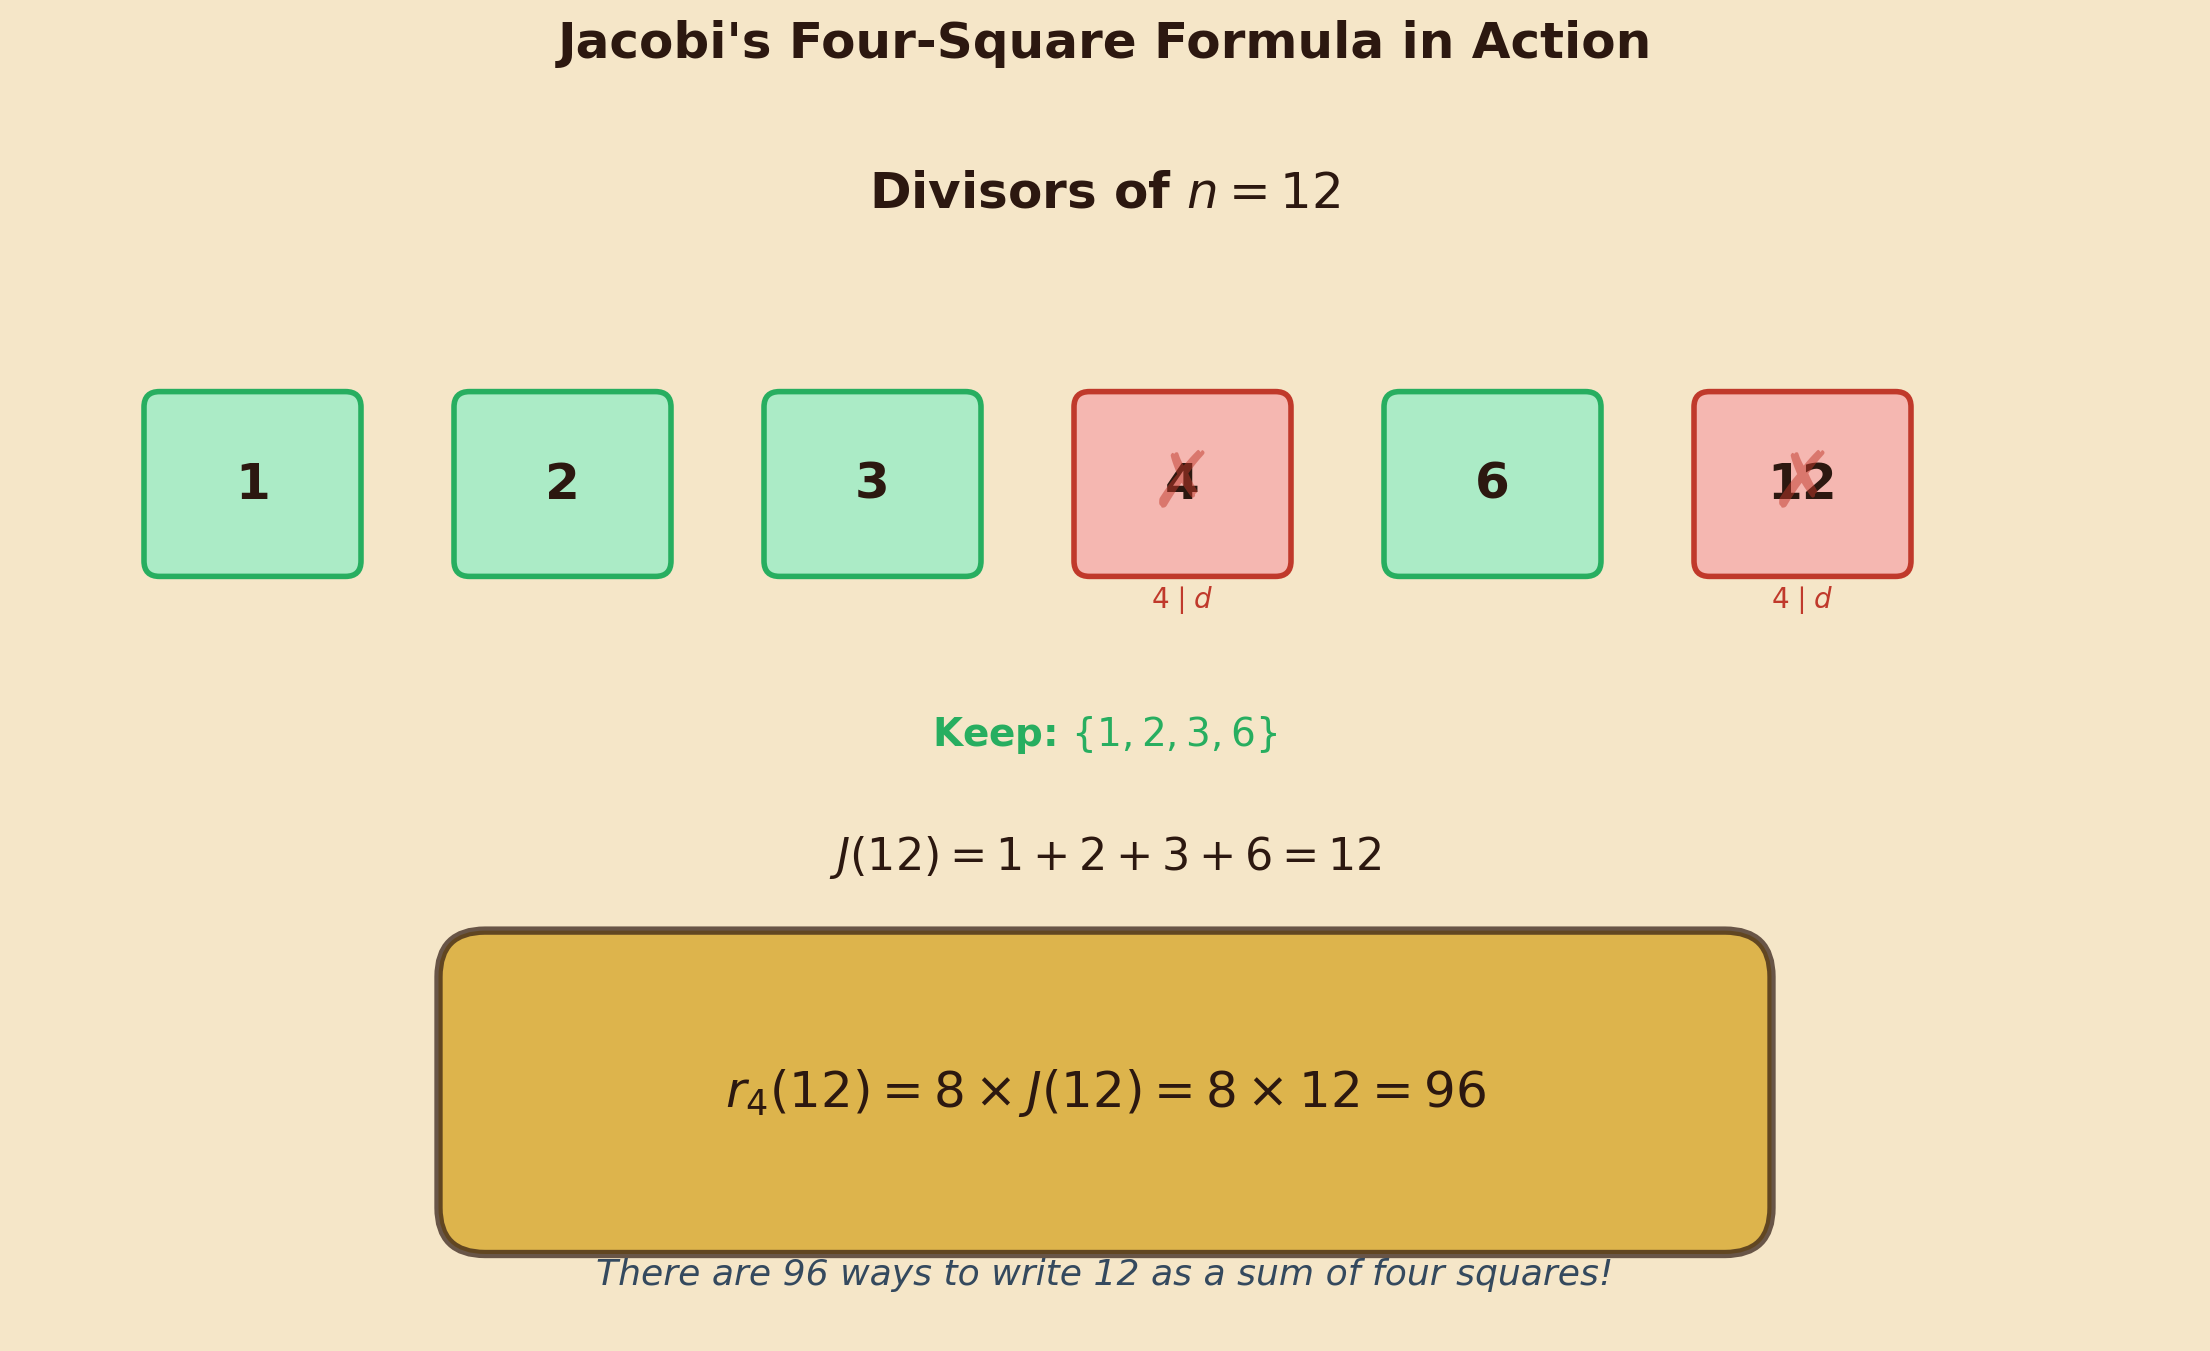
\includegraphics[width=0.82\textwidth,keepaspectratio]{images/chapter9_fig13_jacobi_divisors.png}
\caption{A divisor diagram for $n = 12$.}
\end{figure}


Let us verify our earlier computations. For $n = 1$: $J(1) = 1$, and $8 \times 1 = 8 = r_4(1)$. $\checkmark$ For $n = 2$: $J(2) = 1 + 2 = 3$, and $8 \times 3 = 24 = r_4(2)$. $\checkmark$ For $n = 3$: $J(3) = 1 + 3 = 4$, and $8 \times 4 = 32 = r_4(3)$. $\checkmark$

The formula also handles larger cases with aplomb. For $n = 5$: $r_4(5) = 8 \times 6 = 48$. If you are skeptical, try listing all $48$ quadruples --- you will find exactly $48$, no more and no less. (This is a fine rainy-afternoon exercise.)

\begin{figure}[htbp]
\centering
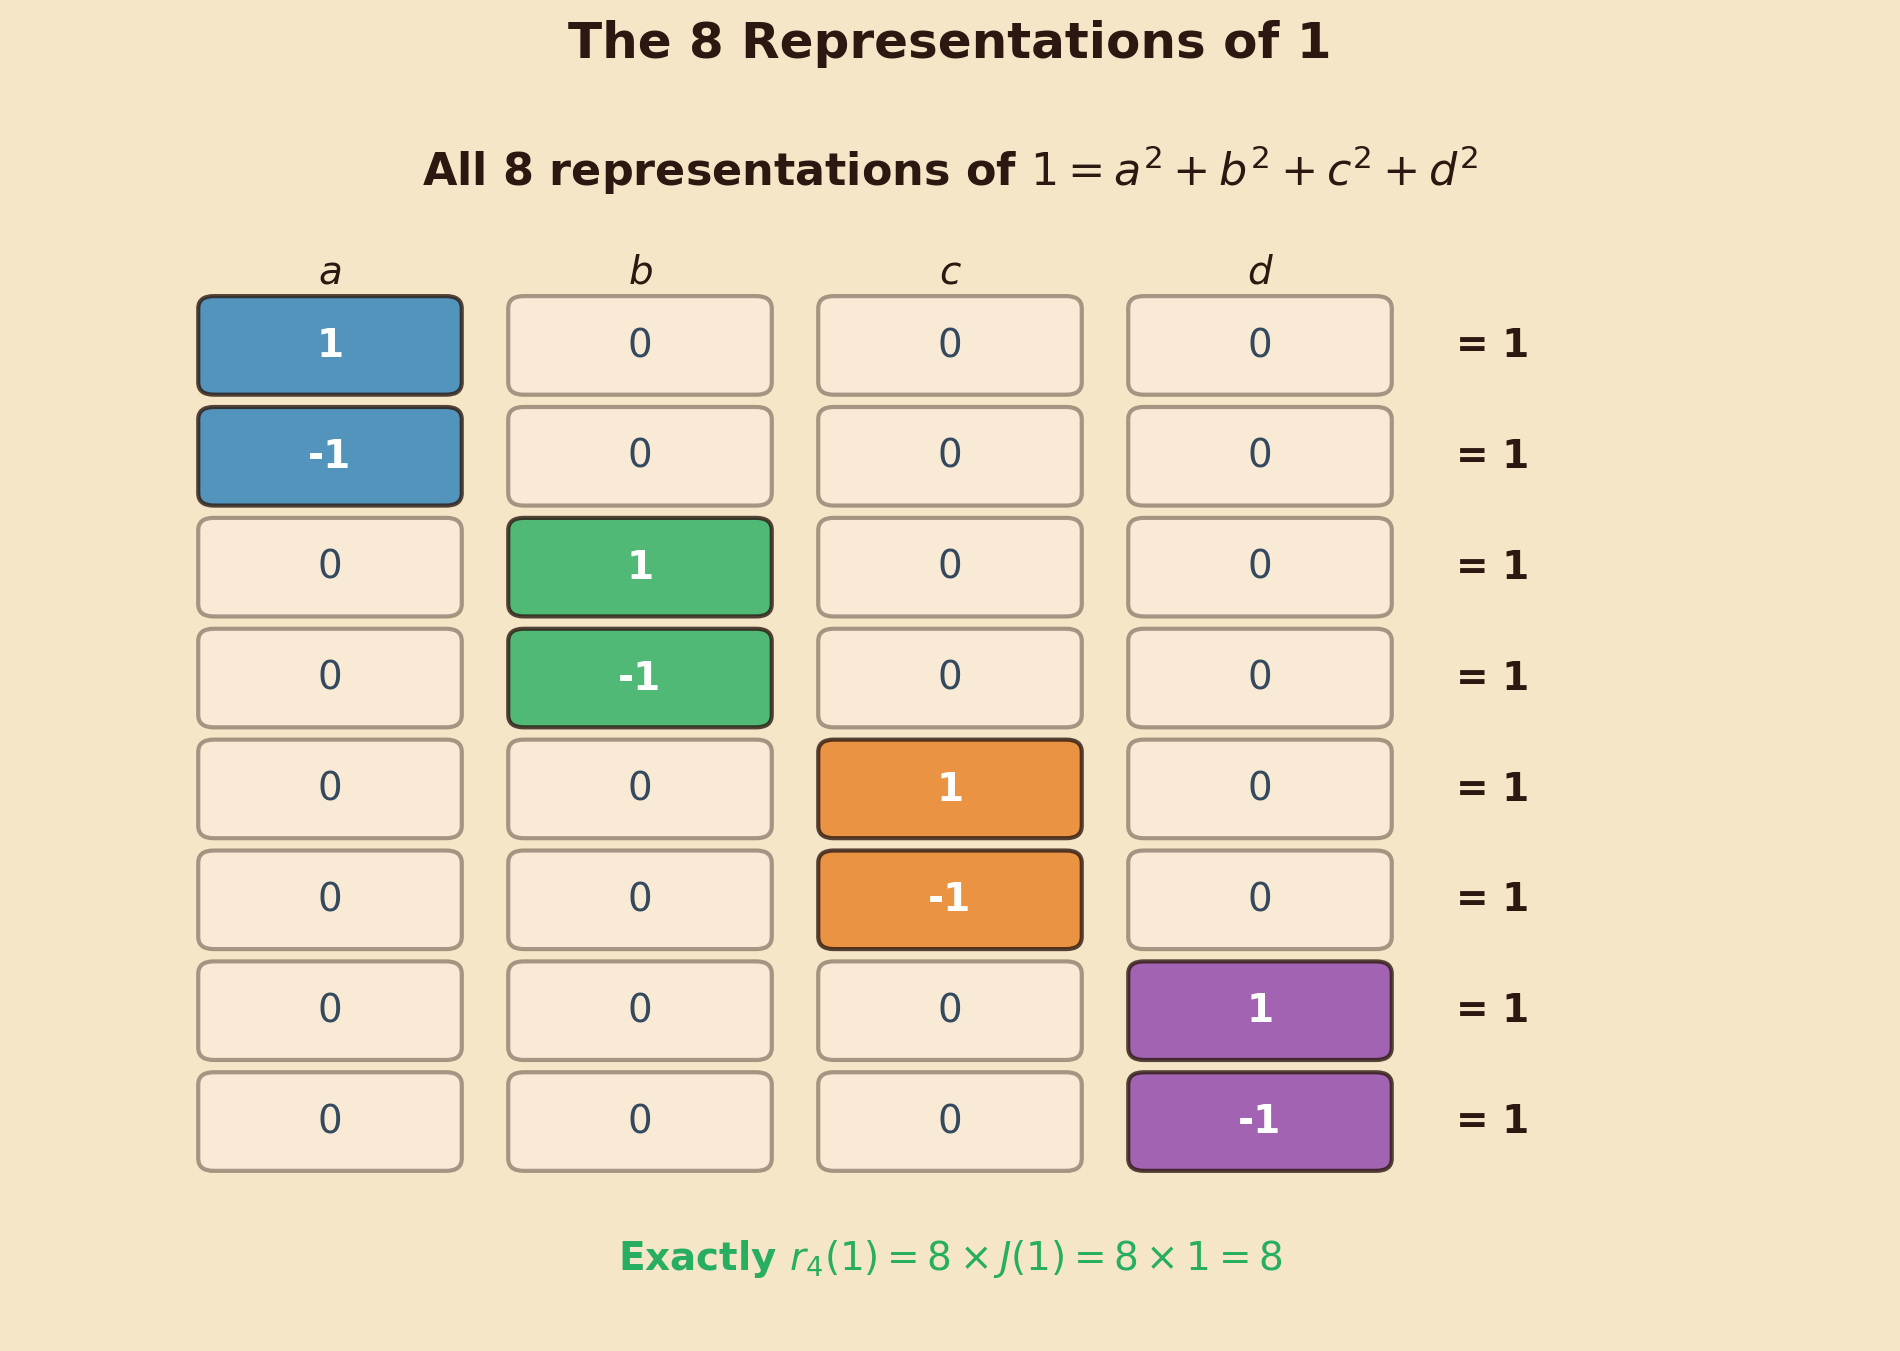
\includegraphics[width=0.82\textwidth,keepaspectratio]{images/chapter9_fig14_representations_of_one.png}
\caption{A visual enumeration of the $8$ representations of $1$ as a sum of four squares.}
\end{figure}


\textbf{An exercise for the reader.} Compute $J(7)$ and use Jacobi's theorem to predict $r_4(7)$. Then verify by finding all the representations. (Hint: the only solution shapes are one $\pm 1$ and one $\pm\sqrt{6}$... but $\sqrt{6}$ is not an integer! So the only shapes are: three entries $\pm 1$ and one entry $\pm 2$, since $1 + 1 + 1 + 4 = 7$. Count carefully.)

Jacobi proved this theorem using the theory of \textit{theta functions} --- the beautiful series $\theta(q) = \sum_{n=-\infty}^{\infty} q^{n^2}$, whose fourth power $\theta(q)^4 = \sum_{n=0}^{\infty} r_4(n)\, q^n$ encodes all the representation numbers at once. The key insight is that $\theta(q)^4$ is a \textit{modular form} of weight $2$ --- a function that transforms in a very particular way under the group of $2 \times 2$ integer matrices --- and the space of such modular forms is so small (one-dimensional, for the relevant level) that $\theta(q)^4$ must equal a certain Eisenstein series, which has the explicit Fourier coefficients $8 \cdot J(n)$. The proof is a masterpiece of the interplay between analysis, algebra, and number theory.

Ramanujan, decades later, would extend this circle of ideas in astonishing directions, discovering exact formulas for $r_k(n)$ for larger values of $k$ and connecting them to his own mysterious modular forms\index{modular forms}. The connection between "counting squares" and "modular symmetry" remains one of the deepest and most active areas of modern number theory.


\ornbreak



\section{The View from the Summit --- Patterns, Paradoxes, and Open Doors}


We have climbed the four-rung ladder from the humble real numbers to the exotic octonions, watching cherished algebraic laws fall away one by one like autumn leaves. Let us pause at the summit and survey the landscape.

Here is the full hierarchy, compressed into a single table:

\begin{center}
\small
\begin{tabular}{lllll}
\toprule
Channel & Algebra & Dimension & Property Lost & Composition Identity \\
\midrule
0 & $\mathbb{R}$ & $1 = 2^0$ & --- & $a^2 \cdot c^2 = (ac)^2$ \\
1 & $\mathbb{C}$ & $2 = 2^1$ & Total ordering & Brahmagupta–Fibonacci \\
2 & $\mathbb{H}$ & $4 = 2^2$ & Commutativity & Euler four-square \\
3 & $\mathbb{O}$ & $8 = 2^3$ & Associativity & Degen eight-square \\
4 & $\mathbb{S}$ & $16 = 2^4$ & Division & $\times$ None \\
\bottomrule
\end{tabular}
\end{center}


\begin{figure}[htbp]
\centering
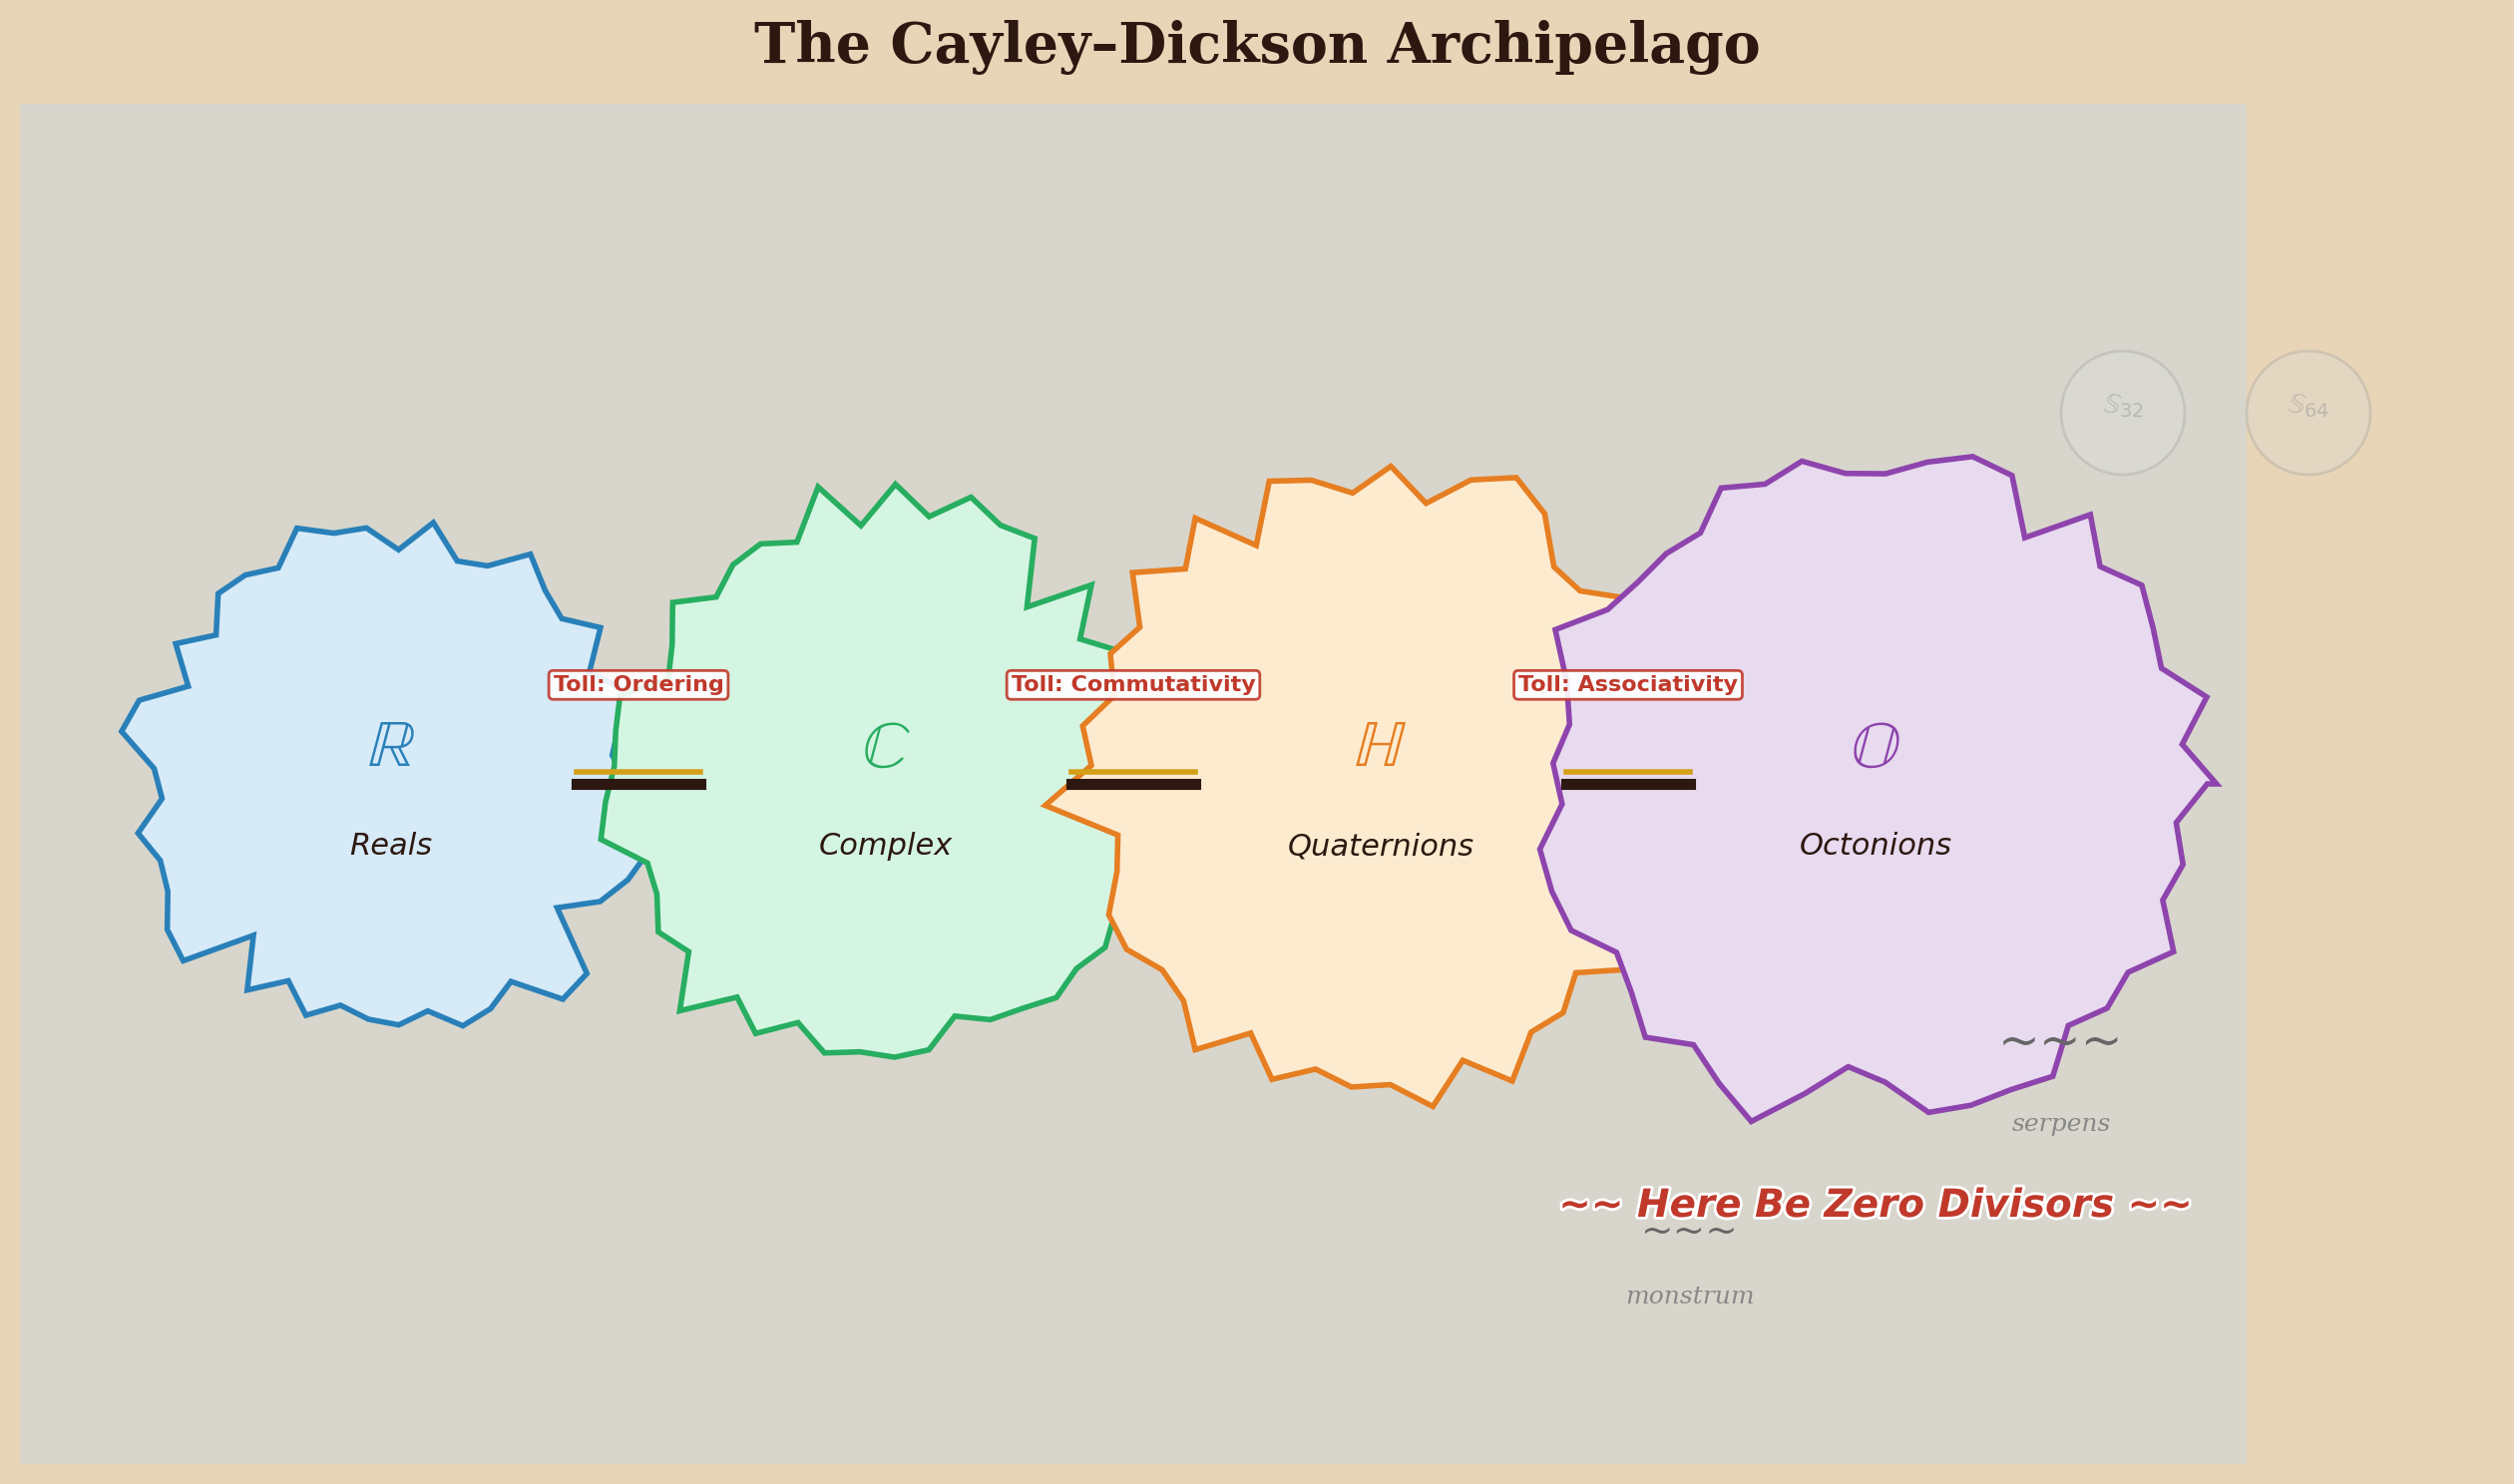
\includegraphics[width=0.82\textwidth,keepaspectratio]{images/chapter9_fig15_cayley_dickson_map.png}
\caption{A full-page "map" of the Cayley–Dickson landscape, drawn in the style of a medieval cartographic illustration.}
\end{figure}


The pattern is seductive. Each rung doubles the dimension and sacrifices one property, gaining expressive power in return. The first four doublings are fertile; the fifth is catastrophic. Why? What makes $16$ the point of no return?

The answer, at its deepest level, involves the topology of spheres and the structure of Clifford algebras. Albrecht Pfister extended the composition story in a different direction: he showed that \textit{Pfister forms} --- certain quadratic forms in $2^n$ variables --- always have the property that if they represent a number, they represent all of its multiples. This is a weaker cousin of the composition property, but it exists in \textit{every} power-of-two dimension. The Hurwitz theorem says the full composition property is restricted to dimensions $1$, $2$, $4$, $8$; the Pfister theorem says a weaker form of multiplicativity persists in all dimensions $2^n$. The four normed division algebras are the special cases where both properties coincide.

The connections to physics are equally tantalizing. The four division algebras appear, unbidden, in the classification of supersymmetric theories: superstring theory can be formulated in $d = 3, 4, 6, 10$ spacetime dimensions, which are $2 + 1$, $3 + 1$, $5 + 1$, $9 + 1$ --- and the "transverse" dimensions in each case are $1, 2, 4, 8$, the dimensions of $\mathbb{R}, \mathbb{C}, \mathbb{H}, \mathbb{O}$. The exceptional Lie groups $G_2$, $F_4$, $E_6$, $E_7$, and $E_8$ --- the "sporadic" symmetries that have puzzled mathematicians since Killing and Cartan classified them --- are all intimately connected to the octonions. Some physicists have even proposed an "octonionic" approach to the Standard Model of particle physics, in which the three generations of quarks and leptons arise from the algebraic structure of $\mathbb{O}$.

\begin{figure}[htbp]
\centering
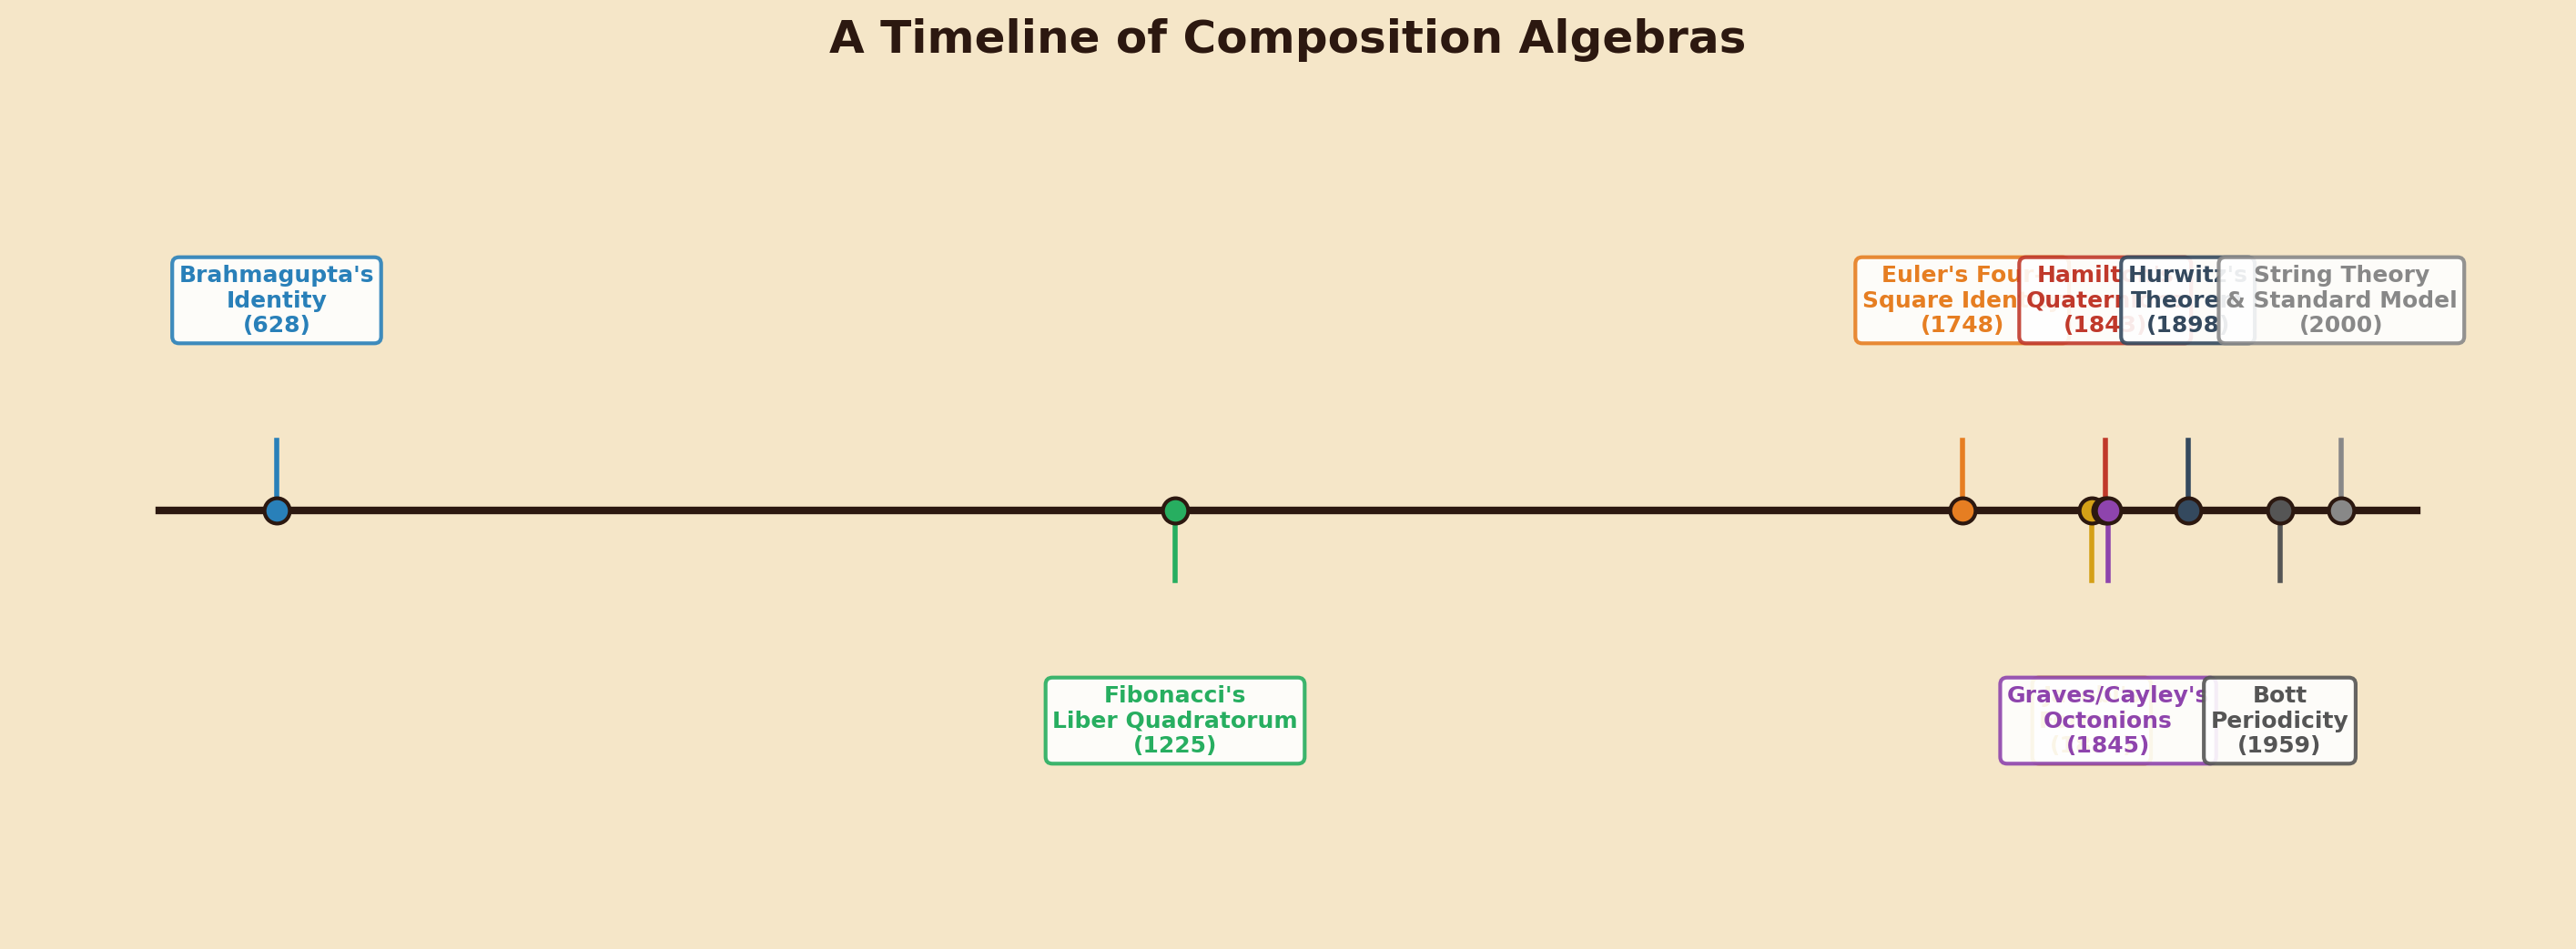
\includegraphics[width=0.82\textwidth,keepaspectratio]{images/chapter9_fig16_timeline.png}
\caption{A timeline spanning from Brahmagupta (628 CE) to the present, marking the key discoveries: Brahmagupta's identity (628), Fibonacci's \textit{Liber Quadratorum} (1225), Euler's four-square identity (1748), Hamilton's quaternions (1843), Graves/Cayley's octonions (1843–1845), Hurwitz's theorem (1898), Bott periodicity (1959), and modern connections to string theory and the Standard Model.}
\end{figure}


Whether the octonions hold the key to fundamental physics, or whether they are merely a beautiful mathematical curiosity with superficial resemblances to the physical world, remains one of the great open questions at the frontier of mathematical physics. What is certain is this: the four normed division algebras --- $\mathbb{R}$, $\mathbb{C}$, $\mathbb{H}$, $\mathbb{O}$ --- are among the most remarkable structures in all of mathematics. They appear, independently and unexpectedly, in algebra, topology, number theory, and physics. Their properties are governed by the interplay of dimension, associativity, commutativity, and divisibility in ways that no one fully understands. And the fact that they correspond exactly to the dimensions where sums-of-squares identities exist --- the Brahmagupta identity for $2$, the Euler identity for $4$, the Degen identity for $8$ --- ties our entire journey through this chapter into a single, luminous thread.

I leave you with a final puzzle, in the spirit of the game we played at the beginning. We have seen that at each rung of the ladder, a law of arithmetic vanishes. At the bottom, we have \textit{everything}: ordering, commutativity, associativity, and division. At the top, we have \textit{almost nothing}: the octonions are not even associative.

But here is what we \textit{gain} at each step: a richer composition identity, a more powerful representation theorem, a deeper connection to the geometry and physics of the world. The ladder exacts a toll --- but it also opens a door. The question is: what lies beyond the door at the top?

That question, dear reader, is still open.


\ornbreak


\textit{Puzzle for the reader (no peeking at the answer!):}

\begin{quote}
\textit{The eight-square identity (Degen's identity) gives an explicit composition law for the octonion norm. It is vastly more complex than Euler's four-square identity, which was already formidable. How many terms appear on the right-hand side of the eight-square identity? And what is the minimum number of minus signs required among those terms? Before computing, try to guess --- the answer may surprise you.}
\end{quote}

